\documentclass[conference]{IEEEtran}
% Some Computer Society conferences also require the compsoc mode option,
% but others use the standard conference format.
%
% If IEEEtran.cls has not been installed into the LaTeX system files,
% manually specify the path to it like:
% \documentclass[conference]{../sty/IEEEtran}



%cmap has to be loaded before any font package (such as cfr-lm)
\usepackage{cmap}
\usepackage[T1]{fontenc}


\usepackage{graphicx,url}
\usepackage[table,xcdraw]{xcolor}

\usepackage{times}
\usepackage{latexsym}
 \usepackage[printonlyused]{acronym}
 
\usepackage{blindtext}
\usepackage{graphicx}
\usepackage{amsmath}
\usepackage{kpfonts}
\usepackage{url}
\usepackage{listings}
\usepackage{multirow}
\usepackage{booktabs} 
\usepackage{pgfplots}
\usepackage{graphicx}
\usepackage{cancel}
\usetikzlibrary{patterns}
\pgfplotsset{width=10cm,compat=1.9}


\usepackage{color}

\usepackage{url}

\usepackage{amsmath}
\usepackage{amssymb}


\acrodef{pots}[POTS]{Poverty of the Stimulus}

\acrodef{CBIR}{Content-based image retrieval}
\acrodef{MAM}{Metric Access Method}
\acrodef{AM}{Access Method}
\acrodef{SAM}{Spatial Access Method}
\acrodef{MST} {Minimum Spanning Tree}
\acrodef{IR} {Information Retrieval}
\acrodef{NDC} {Number of Distance Calculations}
\acrodef{LAESA} {Linear Approximating Eliminating Search Algorithm}
\acrodef{AESA} {Approximating Eliminating Search Algorithm}
\acrodef{RNG} {Relative Neighborhood Graph}
\acrodef{DT} {Delaunay Triangulation}
\acrodef{GG} {Gabriel Graph}
\acrodef{UG} {Urquhart Graph}
\acrodef{SAT} {Spacial Approximation Tree}
\acrodef{RNDF} {Relative Neighborhood Density Factor}
\acrodef{NN} {Nearest Neighbor}
\acrodef{NAG} {Neighborhood Approximation Graph}
\acrodef{HRG} {Hyperspherical Region Graph}
\acrodef{NA-Graph} {Neighborhood Approximation Graph}
\acrodef{DA} {Disk Access}
\acrodef{DTW} {Dynamic Time Warping}
\acrodef{LSH} {Locality Sensitive Hashing}
\acrodef{CNN} {Convolutional Neural Network}
\acrodef{CNNs} {Convolutional Neural Networks}

\usepackage{pgfplotstable,booktabs}
%%%%%%%%%%%%%%%%%%%%%%%%%%%%%%%%%%%%%%%%%%%%%%
%% You don't need this part
% I did it to create your file 
\usepackage{filecontents} % <-- To create files on the fly


% Needed packages
\usepackage{tikz}
\usepackage{pgfplots}
\pgfplotsset{compat=newest}

% Command to read a number from file (the hspace is quite hacky...)
\newcommand{\showodsf}[2]{%
\mbox{\input{data/#1_#2_ods_f.txt}\hspace{-2.5pt}}%
}

\newcommand{ \Correction }[ 1 ] {\textcolor{black}{#1}}
\newcommand{ \NewMaterial }[ 1 ] {\textcolor{black}{#1}}
\newcommand{ \ConnectDots }[ 1 ] {\textcolor{black}{#1}}


%Even though `american`, `english` and `USenglish` are synonyms for babel package (according to https://tex.stackexchange.com/questions/12775/babel-english-american-usenglish), the llncs document class is prepared to avoid the overriding of certain names (such as "Abstract." -> "Abstract" or "Fig." -> "Figure") when using `english`, but not when using the other 2.
%english has to go last to set it as default language
\usepackage[ngerman,english]{babel}
%Hint by http://tex.stackexchange.com/a/321066/9075 -> enable "= as dashes
\addto\extrasenglish{\languageshorthands{ngerman}\useshorthands{"}}

%better font, similar to the default springer font
%cfr-lm is preferred over lmodern. Reasoning at http://tex.stackexchange.com/a/247543/9075
\usepackage[%
rm={oldstyle=false,proportional=true},%
sf={oldstyle=false,proportional=true},%
tt={oldstyle=false,proportional=true,variable=true},%
qt=false%
]{cfr-lm}
 
%for easy quotations: \enquote{text}
\usepackage{csquotes}

%enable margin kerning
\usepackage{microtype}

%tweak \url{...}
\usepackage{url}
%\urlstyle{same}
%improve wrapping of URLs - hint by http://tex.stackexchange.com/a/10419/9075
\makeatletter
\g@addto@macro{\UrlBreaks}{\UrlOrds}
\makeatother
%nicer // - solution by http://tex.stackexchange.com/a/98470/9075
%DO NOT ACTIVATE -> prevents line breaks
%\makeatletter
%\def\Url@twoslashes{\mathchar`\/\@ifnextchar/{\kern-.2em}{}}
%\g@addto@macro\UrlSpecials{\do\/{\Url@twoslashes}}
%\makeatother

%diagonal lines in a table - http://tex.stackexchange.com/questions/17745/diagonal-lines-in-table-cell
%slashbox is not available in texlive (due to licensing) and also gives bad results. This, we use diagbox
%\usepackage{diagbox}

%required for pdfcomment later
\usepackage{xcolor}


%enable nice comments
%this also loads hyperref
\usepackage{pdfcomment}
%enable hyperref without colors and without bookmarks
\hypersetup{hidelinks,
   colorlinks=true,
   allcolors=black,
   pdfstartview=Fit,
   breaklinks=true}
%enables correct jumping to figures when referencing
\usepackage[all]{hypcap}

\newcommand{\commentontext}[2]{\colorbox{yellow!60}{#1}\pdfcomment[color={0.234 0.867 0.211},hoffset=-6pt,voffset=10pt,opacity=0.5]{#2}}
\newcommand{\commentatside}[1]{\pdfcomment[color={0.045 0.278 0.643},icon=Note]{#1}}

%compatibality with packages todo, easy-todo, todonotes
\newcommand{\todo}[1]{\commentatside{#1}}
%compatiblity with package fixmetodonotes
\newcommand{\TODO}[1]{\commentatside{#1}}

%enable \cref{...} and \Cref{...} instead of \ref: Type of reference included in the link
\usepackage[capitalise,nameinlink]{cleveref}
%Nice formats for \cref
\crefname{section}{Sect.}{Sect.}
\Crefname{section}{Section}{Sections}

\usepackage{xspace}
%\newcommand{\eg}{e.\,g.\xspace}
%\newcommand{\ie}{i.\,e.\xspace}
\newcommand{\eg}{e.\,g.,\ }
\newcommand{\ie}{i.\,e.,\ }
% Some very useful LaTeX packages include:
% (uncomment the ones you want to load)


% *** MISC UTILITY PACKAGES ***
%
%\usepackage{ifpdf}
% Heiko Oberdiek's ifpdf.sty is very useful if you need conditional
% compilation based on whether the output is pdf or dvi.
% usage:
% \ifpdf
%   % pdf code
% \else
%   % dvi code
% \fi
% The latest version of ifpdf.sty can be obtained from:
% http://www.ctan.org/pkg/ifpdf
% Also, note that IEEEtran.cls V1.7 and later provides a builtin
% \ifCLASSINFOpdf conditional that works the same way.
% When switching from latex to pdflatex and vice-versa, the compiler may
% have to be run twice to clear warning/error messages.






% *** CITATION PACKAGES ***
%
%\usepackage{cite}
% cite.sty was written by Donald Arseneau
% V1.6 and later of IEEEtran pre-defines the format of the cite.sty package
% \cite{} output to follow that of the IEEE. Loading the cite package will
% result in citation numbers being automatically sorted and properly
% "compressed/ranged". e.g., [1], [9], [2], [7], [5], [6] without using
% cite.sty will become [1], [2], [5]--[7], [9] using cite.sty. cite.sty's
% \cite will automatically add leading space, if needed. Use cite.sty's
% noadjust option (cite.sty V3.8 and later) if you want to turn this off
% such as if a citation ever needs to be enclosed in parenthesis.
% cite.sty is already installed on most LaTeX systems. Be sure and use
% version 5.0 (2009-03-20) and later if using hyperref.sty.
% The latest version can be obtained at:
% http://www.ctan.org/pkg/cite
% The documentation is contained in the cite.sty file itself.






% *** GRAPHICS RELATED PACKAGES ***
%
\ifCLASSINFOpdf
  % \usepackage[pdftex]{graphicx}
  % declare the path(s) where your graphic files are
  % \graphicspath{{../pdf/}{../jpeg/}}
  % and their extensions so you won't have to specify these with
  % every instance of \includegraphics
  % \DeclareGraphicsExtensions{.pdf,.jpeg,.png}
\else
  % or other class option (dvipsone, dvipdf, if not using dvips). graphicx
  % will default to the driver specified in the system graphics.cfg if no
  % driver is specified.
  % \usepackage[dvips]{graphicx}
  % declare the path(s) where your graphic files are
  % \graphicspath{{../eps/}}
  % and their extensions so you won't have to specify these with
  % every instance of \includegraphics
  % \DeclareGraphicsExtensions{.eps}
\fi
% graphicx was written by David Carlisle and Sebastian Rahtz. It is
% required if you want graphics, photos, etc. graphicx.sty is already
% installed on most LaTeX systems. The latest version and documentation
% can be obtained at: 
% http://www.ctan.org/pkg/graphicx
% Another good source of documentation is "Using Imported Graphics in
% LaTeX2e" by Keith Reckdahl which can be found at:
% http://www.ctan.org/pkg/epslatex
%
% latex, and pdflatex in dvi mode, support graphics in encapsulated
% postscript (.eps) format. pdflatex in pdf mode supports graphics
% in .pdf, .jpeg, .png and .mps (metapost) formats. Users should ensure
% that all non-photo figures use a vector format (.eps, .pdf, .mps) and
% not a bitmapped formats (.jpeg, .png). The IEEE frowns on bitmapped formats
% which can result in "jaggedy"/blurry rendering of lines and letters as
% well as large increases in file sizes.
%
% You can find documentation about the pdfTeX application at:
% http://www.tug.org/applications/pdftex





% *** MATH PACKAGES ***
%
%\usepackage{amsmath}
% A popular package from the American Mathematical Society that provides
% many useful and powerful commands for dealing with mathematics.
%
% Note that the amsmath package sets \interdisplaylinepenalty to 10000
% thus preventing page breaks from occurring within multiline equations. Use:
%\interdisplaylinepenalty=2500
% after loading amsmath to restore such page breaks as IEEEtran.cls normally
% does. amsmath.sty is already installed on most LaTeX systems. The latest
% version and documentation can be obtained at:
% http://www.ctan.org/pkg/amsmath





% *** SPECIALIZED LIST PACKAGES ***
%
%\usepackage{algorithmic}
% algorithmic.sty was written by Peter Williams and Rogerio Brito.
% This package provides an algorithmic environment fo describing algorithms.
% You can use the algorithmic environment in-text or within a figure
% environment to provide for a floating algorithm. Do NOT use the algorithm
% floating environment provided by algorithm.sty (by the same authors) or
% algorithm2e.sty (by Christophe Fiorio) as the IEEE does not use dedicated
% algorithm float types and packages that provide these will not provide
% correct IEEE style captions. The latest version and documentation of
% algorithmic.sty can be obtained at:
% http://www.ctan.org/pkg/algorithms
% Also of interest may be the (relatively newer and more customizable)
% algorithmicx.sty package by Szasz Janos:
% http://www.ctan.org/pkg/algorithmicx




% *** ALIGNMENT PACKAGES ***
%
%\usepackage{array}
% Frank Mittelbach's and David Carlisle's array.sty patches and improves
% the standard LaTeX2e array and tabular environments to provide better
% appearance and additional user controls. As the default LaTeX2e table
% generation code is lacking to the point of almost being broken with
% respect to the quality of the end results, all users are strongly
% advised to use an enhanced (at the very least that provided by array.sty)
% set of table tools. array.sty is already installed on most systems. The
% latest version and documentation can be obtained at:
% http://www.ctan.org/pkg/array


% IEEEtran contains the IEEEeqnarray family of commands that can be used to
% generate multiline equations as well as matrices, tables, etc., of high
% quality.




% *** SUBFIGURE PACKAGES ***
%\ifCLASSOPTIONcompsoc
%  \usepackage[caption=false,font=normalsize,labelfont=sf,textfont=sf]{subfig}
%\else
%  \usepackage[caption=false,font=footnotesize]{subfig}
%\fi
% subfig.sty, written by Steven Douglas Cochran, is the modern replacement
% for subfigure.sty, the latter of which is no longer maintained and is
% incompatible with some LaTeX packages including fixltx2e. However,
% subfig.sty requires and automatically loads Axel Sommerfeldt's caption.sty
% which will override IEEEtran.cls' handling of captions and this will result
% in non-IEEE style figure/table captions. To prevent this problem, be sure
% and invoke subfig.sty's "caption=false" package option (available since
% subfig.sty version 1.3, 2005/06/28) as this is will preserve IEEEtran.cls
% handling of captions.
% Note that the Computer Society format requires a larger sans serif font
% than the serif footnote size font used in traditional IEEE formatting
% and thus the need to invoke different subfig.sty package options depending
% on whether compsoc mode has been enabled.
%
% The latest version and documentation of subfig.sty can be obtained at:
% http://www.ctan.org/pkg/subfig




% *** FLOAT PACKAGES ***
%
%\usepackage{fixltx2e}
% fixltx2e, the successor to the earlier fix2col.sty, was written by
% Frank Mittelbach and David Carlisle. This package corrects a few problems
% in the LaTeX2e kernel, the most notable of which is that in current
% LaTeX2e releases, the ordering of single and double column floats is not
% guaranteed to be preserved. Thus, an unpatched LaTeX2e can allow a
% single column figure to be placed prior to an earlier double column
% figure.
% Be aware that LaTeX2e kernels dated 2015 and later have fixltx2e.sty's
% corrections already built into the system in which case a warning will
% be issued if an attempt is made to load fixltx2e.sty as it is no longer
% needed.
% The latest version and documentation can be found at:
% http://www.ctan.org/pkg/fixltx2e


%\usepackage{stfloats}
% stfloats.sty was written by Sigitas Tolusis. This package gives LaTeX2e
% the ability to do double column floats at the bottom of the page as well
% as the top. (e.g., "\begin{figure*}[!b]" is not normally possible in
% LaTeX2e). It also provides a command:
%\fnbelowfloat
% to enable the placement of footnotes below bottom floats (the standard
% LaTeX2e kernel puts them above bottom floats). This is an invasive package
% which rewrites many portions of the LaTeX2e float routines. It may not work
% with other packages that modify the LaTeX2e float routines. The latest
% version and documentation can be obtained at:
% http://www.ctan.org/pkg/stfloats
% Do not use the stfloats baselinefloat ability as the IEEE does not allow
% \baselineskip to stretch. Authors submitting work to the IEEE should note
% that the IEEE rarely uses double column equations and that authors should try
% to avoid such use. Do not be tempted to use the cuted.sty or midfloat.sty
% packages (also by Sigitas Tolusis) as the IEEE does not format its papers in
% such ways.
% Do not attempt to use stfloats with fixltx2e as they are incompatible.
% Instead, use Morten Hogholm'a dblfloatfix which combines the features
% of both fixltx2e and stfloats:
%
% \usepackage{dblfloatfix}
% The latest version can be found at:
% http://www.ctan.org/pkg/dblfloatfix




% *** PDF, URL AND HYPERLINK PACKAGES ***
%
%\usepackage{url}
% url.sty was written by Donald Arseneau. It provides better support for
% handling and breaking URLs. url.sty is already installed on most LaTeX
% systems. The latest version and documentation can be obtained at:
% http://www.ctan.org/pkg/url
% Basically, \url{my_url_here}.




% *** Do not adjust lengths that control margins, column widths, etc. ***
% *** Do not use packages that alter fonts (such as pslatex).         ***
% There should be no need to do such things with IEEEtran.cls V1.6 and later.
% (Unless specifically asked to do so by the journal or conference you plan
% to submit to, of course. )


% correct bad hyphenation here
\hyphenation{op-tical net-works semi-conduc-tor}


\begin{document}
%
% paper title
% Titles are generally capitalized except for words such as a, an, and, as,
% at, but, by, for, in, nor, of, on, or, the, to and up, which are usually
% not capitalized unless they are the first or last word of the title.
% Linebreaks \\ can be used within to get better formatting as desired.
% Do not put math or special symbols in the title.
\title{Approximate nearest neighbors by  deep learning hashing on large-scale search}

% author names and affiliations
% use a multiple column layout for up to three different
% affiliations
\author{\IEEEauthorblockN{Michael Shell}
\IEEEauthorblockA{School of Electrical and\\Computer Engineering\\
Georgia Institute of Technology\\
Atlanta, Georgia 30332--0250\\
Email: http://www.michaelshell.org/contact.html}
\and
\IEEEauthorblockN{James Kirk\\ and Montgomery Scott}
\IEEEauthorblockA{Starfleet Academy\\
San Francisco, California 96678--2391\\
Telephone: (800) 555--1212\\
Fax: (888) 555--1212}}

% conference papers do not typically use \thanks and this command
% is locked out in conference mode. If really needed, such as for
% the acknowledgment of grants, issue a \IEEEoverridecommandlockouts
% after \documentclass

% for over three affiliations, or if they all won't fit within the width
% of the page, use this alternative format:
% 
%\author{\IEEEauthorblockN{Michael Shell\IEEEauthorrefmark{1},
%Homer Simpson\IEEEauthorrefmark{2},
%James Kirk\IEEEauthorrefmark{3}, 
%Montgomery Scott\IEEEauthorrefmark{3} and
%Eldon Tyrell\IEEEauthorrefmark{4}}
%\IEEEauthorblockA{\IEEEauthorrefmark{1}School of Electrical and Computer Engineering\\
%Georgia Institute of Technology,
%Atlanta, Georgia 30332--0250\\ Email: see http://www.michaelshell.org/contact.html}
%\IEEEauthorblockA{\IEEEauthorrefmark{2}Twentieth Century Fox, Springfield, USA\\
%Email: homer@thesimpsons.com}
%\IEEEauthorblockA{\IEEEauthorrefmark{3}Starfleet Academy, San Francisco, California 96678-2391\\
%Telephone: (800) 555--1212, Fax: (888) 555--1212}
%\IEEEauthorblockA{\IEEEauthorrefmark{4}Tyrell Inc., 123 Replicant Street, Los Angeles, California 90210--4321}}




% use for special paper notices
%\IEEEspecialpapernotice{(Invited Paper)}




% make the title area
\maketitle

% As a general rule, do not put math, special symbols or citations
% in the abstract
\begin{abstract}

An optimal data representation  is  an important  task in information retrieval.   A fast indexing method increases the performance level and a good representation offers precise discrimination.  

%In this work we perform exhaustive experiments  
    

In this Similarity search algorithms based on hashing were proposed to query high-dimensional datasets due to its fast retrieval speed and low storage cost.   Recent studies, promote the use of  \ac{CNN} with hashing techniques to improve the search accuracy.  However, there are challenges to solve in order to find a practical and efficient solution to index CNN features, such as the need for heavy training process to achieve accurate query results and the critical dependency on data-parameters.   Aiming to overcome these issues, we propose a new method for scalable similarity search, i.e., Deep frActal based  Hashing (DAsH), by computing the best data-parameters values for optimal sub-space projection  exploring the correlations among CNN features attributes using fractal theory. Moreover, inspired by recent advances in CNNs, we use not only activations of lower layers which are more general-purpose but also previous knowledge of the semantic data on the latest CNN layer to improve the search accuracy.  Thus, our method produces a better representation of the data space with a less computational cost for a better accuracy.  This significant gain in speed and accuracy allows us to evaluate the framework on a  large, realistic, and challenging set of datasets.  

\end{abstract}

% no keywords




% For peer review papers, you can put extra information on the cover
% page as needed:
% \ifCLASSOPTIONpeerreview
% \begin{center} \bfseries EDICS Category: 3-BBND \end{center}
% \fi
%
% For peerreview papers, this IEEEtran command inserts a page break and
% creates the second title. It will be ignored for other modes.
\IEEEpeerreviewmaketitle




\section{Introduction}\label{sec:intro}

The increasing availability of data in diverse domains has created a necessity to develop techniques and methods to discover knowledge from massive volumes of complex data, motivating many research works in databases, machine learning, and information retrieval communities.  This has driven the development of scalable and efficient techniques to organize and retrieve this kind of data. Similarity search has been the traditional approach for information retrieval.  Although several similarity search algorithms have been proposed to speed up similarity queries, most of them are either affected by the well-known ``curse of dimensionality''.  Retrieve  complex data causes   stability problems  when the data dimensionality is very high \cite{aleman_high_dimensional}.  %Some studies have shown that the idea of data representation with hyper spherical or rectangular region hierarchies can deteriorate similarity queries even compared with sequential search \cite{aleman_high_dimensional}.

%Considering that similarity is the instinctive criterion by which people make comparisons, the information retrieval communities use similarity to organize and search for data.    However, even though similarity is an intuitive measure for comparisons, it causes some difficulties on representing complex data and with the stability of the algorithms when the data dimensionality is very high (the ``curse of dimensionality'').  Although many research works have been conducted on developing efficient index structures and similarity search algorithms, only a few of them present theoretical guaranty of asymptotic stability for high-dimensional data.

%% WHAT'S WRONG WITH TREES & CURSE OF HIGH DIMENSIONALITY DATA (mine)
%Many solutions response similarity queries taking advantage of index structures. Trees are the most common index structures for these domains. These solutions based on hierarchies can be overcome by sequential search. The main reason is that, in high dimensional data, most of the time spent during the search process is the filtering step in which it ensures that the current result is the correct answer \cite{WhatsWrong}. Not all applications require accurate answers. Hence,  most of the time approximate solutions are  preferable to reduce the effects of the ``curse of dimensionality''. These approximate solutions are applied in large-scale problems where speed is more important than accuracy. In this context, we need to needs to optimize the balance between time and query result quality.   

One of the few approaches that ensure an approximate solution with sublinear search cost for high-dimensional data is the Locality Sensitive Hashing (LSH) \cite{hashing_algoritghms_survey}. LSH is based on the idea that closeness between two objects is usually preserved by a random projection operation. In other words, if two objects are close together in their original space, then these two objects will remain close after a scalar projection operation. However, it presents some difficulties for approximate kNN queries, in particular, related to data domain parameter dependence and quality results. Therefore, in complex domains, in particular, in high dimensional data problems, an approximate solution with a solid theoretical analysis may be the best option in many application areas because of their efficiency in time and space.


 %% LSH 
% Different approaches have been studied to solve the ``curse of dimensionality''. One of the research lines is to try to avoid the dimensionality problem by relaxing the query precision to speed up the query time. Potentially, this approach is feasible for applications that do not require exact answers and for which speed is more important than search accuracy. Moreover, the metric space definition already leads to an approximation of the true answer, and thus a second approximation at search time may be acceptable \cite{cit:avez99searching}.  
 


 %In this direction, \acf{LSH} \cite{lsh} is one of the recent hash-based techniques proposed to organize and query high-dimensional data. Indeed, LSH is one of the few techniques that provide solid theoretical analysis and predictable loss of accuracy in the results. To answer similarity queries, \ac{LSH} searches only regions, which are represented by buckets, to which the query object is hashed (i.e., the candidate buckets containing the dataset objects with a high probability of similarity to the query object). Therefore, there is no need to fully explore the index data, and only the objects into the candidate buckets require further processing.  

%% CNN %% 

On the other hand, in Machine Learning traditionally images are often described by the hand-craft visual features.  However, these hand-craft features cannot well reveal the high-level semantic meaning (labels or tags) of images, and often limit the performance of image retrieval \cite{Li:2015:RSS:2881665.2882186}.   Inspired by recent advances in \acf{CNN}  \cite{ImageNet}, many methods solved the problem of precision of similarity retrieval by using CNN  as feature extractor and then  build a compact similarity-preserving hash code for fast image retrieval.   Again, hashing is widely used for large-scale image retrieval as well as video and document searches because the compact representation of hash code is essential for data storage and reasonable for query searches \cite{conf/cvpr/ShenSLS15}.  However, some drawbacks based  on these supervised hashing methods have not been solved entirely, as follows:



%We distinguish three classes of methods for supervised hash- ing: triplet loss hashing [1, 2, 3, 4], pairwise similarity-based and label-based. Often, pairwise similarity and label infor- mation are equivalent, because pairwise similarity is defined as sharing the same label, and reciprocally labels are equiv- alence classes of pairwise similarity relations. However they are treated differently because constructing pairwise similar- ity matrices scales quadratically with the number of labeled samples, limiting these algorithms to small labeled sets.


%In a recent work, \cite{kLin:DH} a supervised hashing method trains the model with a binary-like hidden layer as features for image classification tasks. By coupling image features extraction and binary code learning, these methods have shown greatly improved retrieval accuracy. However, some drawbacks based  on these supervised hashing methods have not been solved entirely, as follows:
 
 
 %Nevertheless, there still exist some shortcomings with the training objectives of these methods that limit their practical retrieval performance, as will detailed in our experiments. In addition, the non-linear activations they employ to approximate the quantization step operate at the cost of possibly slowing down the network training \cite{Krizhevsky:2012:ImageNet}.
 
\begin{itemize}


%\item[-]  These supervised  hashing methods \cite{Xia:2014:SHI:2892753.2892851,kLin:DH}  use    non-linear activations, e.g. tang or sigmoid,  to approximate the quantization step. These methods are likely to slow down the training process \cite{ImageNet}.

\item[-]  There is a trade-off between classification error and quantization error: activations of lower layers are more general-purpose \cite{DBLP:journals/corr/YosinskiCBL14}, so training is more effective. However lower layers have larger  activations maps (many nodes), which are harder to encode which leads to a compromise. 
	
%\item[-] In many real applications, it is not easy to decide the appropriate domain parameters at the beginning because the data and query distribution may change during the execution.An approximate similarity search scheme based on hashing cannot handle this dynamic workload because the parameters are tuned for a static dataset.

\item[-]  There is a dependency on parameter values  for approximate similarity search schemes based on LSH, which determine the number of hash functions and number of hash tables.  
 
\end{itemize}

     
%Inspired by recent advances in convolutional neural networks, we propose a novel approach that can utilize  previous knowledge of the semantic data. When semantic information and a related multi-level structure are available, significant improvements can be attained. Exploiting  relationship between semantic and hashing data is the most important thing for large-scale issues. Binary code can be learned from deep neural network for representing the latent concepts that dominate the semantic labels. 
 
 This paper proposes a novel supervised hashing technique,  named  Deep frActal based  Hashing (DAsH),  designed to perform scalable approximate similarity search. The contributions of our work are as follows. First,  we introduce and define a  scheme based on CNN and optimized using fractal theory. To overcome the limitation of large activations on lower layers of CNN (output of the last convolutional layer) we reduce its dimensionality using autoencoders  to the optimal sub-space. Then we index this new representation with LSH scheme.  Second, we present a novel method, based on fractal theory, which allow us to can find the optimal number of hash functions for an approximate similarity search scheme based on LSH.
 
 %  which, as we mentioned, it is also tuned thank to fractal theory

 
% The optimal sub-space projection algorithm based on fractal dimension allow us to use the output the last convolutional layer in combination with autoencoder networks to encode the data to the best sub-space.  We are focused on minimizing the loss of information.  Then we index this new representation with LSH scheme which, as we mentioned, it is also tuned thank to fractal theory.  
  
  
% We find the best data-parameters values by exploring the correlations among CNN features attributes using fractal dimension. Moreover, inspired by recent advances in convolutional neural networks, we use not only activations of lower layers which are more general-purpose but also previous knowledge of the semantic data on latest CNN layers.  Thus, our method produces a better representation of the data space with a less computational cost for a better accuracy.  This significant gain in speed and accuracy allows us to evaluate the framework on a  large, realistic, and challenging set of datasets.  

  
% of lower layers which are more general-purpose but also previous knowledge of the semantic data on latest CNN layers.  Thus, our method produces a better representation of the data space with a less computational cost for a better accuracy.  This significant gain in speed and accuracy allows us to evaluate the framework on a  large, realistic, and challenging set of datasets.  
 
 %  Deep Learning approach can speed improve the accuracy for query process by simultaneously learning feature representations of images, hash codes, and classifiers. Thus, our method produces a better representation of the data space with a less computational cost for training process and a better performance regarding speed and accuracy for query process. 
 
 
%Inspired by recent advances in  \acf{CNNs}, our scheme can utilize not only activations of lower layers which are more general-purpose but also previous knowledge of the semantic data on last CNN layers.    Our scheme can index CNN features using hashing techniques  without the data-parameters dependency problem  exploring the correlations among CNN features attributes by computing the fractal dimension to find the best data-parameters values.   Experimental studies on large   datasets show the similarity search performance in terms of speed and accuracy of the proposed technique.

%%
%Our contributions are as follows. First, we introduce and define a multi-resolution index structure designed to handle a dynamic set of objects. Second, we exploit the multi-resolution approach to speed up similarity queries. Finally, we present our Adaptive Multi-Level LSH algorithms and report experiments on real and synthetic datasets, comparing our approach to recent MAMs and current LSH extensions. To the best of our knowledge, this is the first work that reports a complete performance study comparing state-of-the-art MAMs and LSH indexing techniques.
 

%Approximate similarity  search  algorithms  based on hashing  were  proposed to query high-dimensional datasets due to its fast retrieval speed and low storage cost.   Recent studies, promote the use of  \ac{CNN} with hashing techniques to improve the search accuracy.  However, there are challenges to solve in order to find a practical and efficient solution to index CNN features, such as the need  of heavy training process to achieve accurate query results and the critical dependency on data-parameters values.   Aiming to overcome these issues, we propose a new method  for scalable  similarity search, i.e., Deep frActal based  Hashing (DAsH),  \NewMaterial{by simultaneously learning feature representations of images, hash codes and classifiers}.  We find the best data-parameters values by exploring the correlations among CNN features attributes using  fractal dimension. Moreover, inspired by recent advances in convolutional neural networks, we  use  not only activations of lower layers which are more general-purpose but also previous knowledge of the semantic data on last CNN layers.  Thus, our method  produce a better representation of the data space with a less computational cost for a better accuracy.  This significant gain in speed and accuracy   allows us to evaluate the framework on a  large, realistic, and challenging set of datasets. %Experimental studies on large real and synthetic datasets show the similarity search performance in speed and accuracy of the prsposed technique.

  
%The performance of most existing hashing methods often depends on the used visual features. Traditionally, face image are often described by the hand-craft visual features  However, these hand-craft features cannot well reveal the semantic information of   images, and often limit the performance of face image retrieval.  Therefore, some other hashing methods are proposed to use other better features, such as Convolutional Neural Network (CNN) features. Deep learning to hash methods have shown that both feature representation and hash coding can be learned more effectively using deep neural networks, which can naturally encode any nonlinear hashing functions.   

%% new info about the paper  
%\Correction{This paper proposes a novel hashing technique, named Adaptive Multi-Level LSH, designed to perform approximate similarity search on dynamic datasets. Our technique is based on the idea of LSH of hashing similar objects to the same bucket, but unlike LSH it does not expect the data domain parameters. Hence, we do not need the complete dataset to define the search space. Instead, we dynamically adapt the data domain parameters during the indexing process thanks to the self-adaptive abilities of a multi-resolution index structure (see details in Section \ref{sec:LSH}). Additionally, the multi-resolution approach can speed up the query process.}

%\NewMaterial{Our contributions are as follows. First, we introduce and define a multi-resolution index structure designed to handle a dynamic set of objects.  Second, we exploit the multi-resolution approach to speed up similarity queries. Finally, we present our Adaptive Multi-Level LSH algorithms and report experiments on real and synthetic datasets, comparing our approach to recent MAMs and current LSH extensions. To the best of our knowledge, this is the first work that reports a complete performance study comparing state-of-the-art MAMs and LSH indexing techniques.}

The paper is organized as follows. Section 2 summarizes the background for this work. Section 3 describes the proposed technique and Section 4 reports experimental results on real and synthetic datasets. Finally, we conclude in Section 5.
 
%  In this context, this article proposes a new framework called Evolving Fractal-based Clustering of Data Streams, which is an extension of the work [Bones et al. 2015]. The main module is a novel method for clustering multivariate data streams, based on the calculation of fractal dimension. Our method utilizes the fractal dimension, calculated for data streams that have more than one attribute, to cluster data streams that behave similarly along the time. 




%\section{Definition and Background}\label{sec:background}

%This section presents the preliminary concepts related to this work. First of all it is necessary to define a universe of objects $\mathbb{U}$ and a function $d: \mathbb{U} \times \mathbb{U} \rightarrow \mathbf{R}$ that measures the distance between two objects of $\mathbb{U} $. On metric spaces, $S \subseteq \mathbb{U}$ is a finite set of data that can be preprocessed, where the function $d()$ measures the dissimilarity between objects and satisfies the following properties, $\forall x, y, z \in \mathbb{U}$:  $d(x, y) \geq 0$  (positiveness);  $d(x, y) = d(y, x)$  (symmetry); $d(x, y) = 0 \leftrightarrow x = y$  (reflexivity); $d(x, y) \leq d(x, z) + d(y, z)$  (triangle inequality).  Metrics are fundamental to create access methods to index a dataset, the so-called Metric Access Methods (MAMs) work on metric spaces, organizing data according to a similarity criterion.

%The nearest neighbor problem, which finds the closest point into a dataset to a specified query point, is important in many areas of computer science. We define four nearest neighbor search problems, which we will use in testing our implementation. Given a query object $q \in \mathbb{U}$, in order to recover similar objects to $q$, the following basic types of queries are defined:
%\begin{itemize}
%\item[-] \textbf{Range query $Rq(q, r)$}: finds all elements within the query radius $r$, i.e., $Rq(q, r) = \{ u \in \mathbb{U} | d(u, q) \leq r \}$.

%\item[-] \textbf{k-Nearest Neighbor query $kNN(q, k)$:} finds the $k$ nearest neighbors of $q$, i.e., find a set $A \subseteq \mathbb{U} $ so that $|A| = k$ and $\forall u \in A, v \in \mathbb{U} -  A, d(q, u) \leq d(q, v)$.

%\item[-] \textbf{Approximate Nearest Neighbor query $ANN(q, \varepsilon)$:}  finds the approximate closest neighbors of $q$.  The answer is approximately correct with certain probability, i.e., the success probability $\delta = 1 - \varepsilon$.  There is always a small chance that another object (the true solution) is closer.   
   
%\end{itemize}
 %\begin{itemize}
  %  \item[-] \textbf{Approximate Range Query $(1 + \varepsilon)$-$Rq(q, r)$:} Query which aims to retrieve objects whose distance to the query object $q$ is at most $(1 + \varepsilon) \times r$, where $r$ is the query radius.
  %  \item[-] \textbf{Approximate kNN Query $(1 + \varepsilon)$-$kNN(q, k)$:} Let $\xi$  the distance between the query and the furthest of the true k nearest neighbours.  The $(1+\varepsilon)-kNNq$  search for the k elements most similar to $q$. Suppose that  $S' = \{s_1', s_2', ..., s_k'\}$  is the query result set, then  $\forall s_i' \in S', d(q, s_i') \leq (1 + \varepsilon) \times \xi $
  %  \end{itemize}


%In order to improve the performance of similarity queries, different indexing approaches have been proposed. Metric Access Methods (MAMs) work on metric spaces, organizing data according to a similarity criterion.  Many \acp{MAM}, such as tree-based techniques VP-Tree \cite{VPT}, SAT \cite{SATree}, M-Tree \cite{MTree} and their extensions Slim-Tree \cite{SlimTree}, DBM-Tree \cite{DBMTree} and  DF-Tree \cite{dftree} are found in the literature. Good surveys on \acp{MAM} can be found in \cite{cit:avez99searching,cit:indexDriven}.
 
%Spatial Access Methods (SAM), such as Kd-Tree \cite{kdt}, R-tree \cite{RTreeOriginal} or methods based on them such as R*-Tree \cite{rstartree}, R+-Tree \cite{rplustree}, X-Tree \cite{xtree}, describe the input data as dimensional vectors $(x_1, x_2, ..., x_n)$. They can index points and geometrical objects. Good survey on \acp{SAM} can be found in \cite{Gaede98multidimensional}.

%Recently, a promising indexing technique named Locality Sensitive Hashing (LSH) \cite{lsh_hamming,lsh} was proposed to solve the approximate similarity search in high dimensional data efficiently. \Correction{LSH is based on the idea that  closeness between two objects is usually preserved by a projection operation. In other words, if two objects are close together in their original space, then these two objects will remain close after a scalar projection operation.}

%\NewMaterial{Figure \ref{fig:search_model} illustrates similarity search models for both MAM and LSH approaches.  Figure \ref{fig:search_model} (a) shows the unified model for searching on metric spaces presented in \cite{cit:avez99searching}. A \textit{metric index} organizes the dataset into regions defined by the distance function, such that each region includes objects which are sufficiently close to each other. At the query time, the triangle inequality is applied to discard regions which do not overlap the query region (sphere in the figure). Hence, only the objects in the qualifying regions (gray regions in the figure) are further processed in order to test the query condition.
%}\NewMaterial{A similar search model for \ac{LSH} is shown in Figure \ref{fig:search_model} (b), where each index is defined by a set of hash functions ($H_1, H_2, H_3$) which generate three different partitioning of the search space. Hence, each partitioning is associated to a hash table and its corresponding set of hash functions. Each set of hash functions is employed to organize the dataset into regions of the search space such that objects in the same region are considered close together under certain probability. At the time query, the query object is hashed (using each of the three sets of hash functions - one for each partitioning) to regions with high probability of finding similar objects (all regions in the figure). Finally, the qualifying regions are analyzed in order to report only the objects which satisfy the query condition.}

%\begin{figure}[htp]
%\includegraphics[width=0.41\columnwidth]{mestrado/mam-search-model.pdf}%\label{fig:slimbe:a}
%\includegraphics[width=0.41\columnwidth]{mestrado/lsh_basic_gray.pdf}%\label{fig:slimbe:a}

%\caption{Unified model for searching. (a) Metric Access Methods [search in candidate regions]. (b) LSH [search in subspaces]. }\label{fig:search_model}
%\end{figure}


%\section{Definition and Background}\label{sec:background}

\section{Locality Sensitive Hashing}\label{sec:background}

Previous work \cite{hashing_algoritghms_survey} has explored the idea of hashing objects and grouping them into buckets with the goal of performing approximate similarity search within buckets associated with the query element.  The idea behind LSH is that if two objects are close together in their original space, then these two objects will remain close after a scalar projection operation. Hence, let $h(x)$ be a hash function that maps a d-dimensional point $x$ to a one-dimensional value. The function $h(x)$ is said to be \textit{locality sensitive} if the probability of mapping two d-dimensional points $x_1$, $x_2$ to the same value grows as their distance $d(x_1, x_2)$ decreases.  
%The intuition behind the hash functions is as follows: the dot product  ${a} \cdot {x} $ project each vector to the real line. It follows from $p$-stability that for two vectors $({v_1}, {v_2})$ the distance between their projections $(\vec{a} \cdot \vec{v_1} - \vec{a} \cdot \vec{v_2})$ is distributed as $\parallel v_1 - v_2 \parallel_p X$, where $X$ is a $p$-stable distribution.  

%Let $f_p(t)$ denote the probability density function of the absolute value of the $p$-stable distribution, and $c = \parallel v_1 - v_2\parallel_p$, the probability of collision $p(c)$ is defined as.

%\begin{equation}\label{eq:lsh_df}
%p(c) = Pr[h(v_1) = h(v_2)] = \int_0^w \frac{1}{c} f_p(\frac{t}{c}) (1-\frac{t}{w})\,dt
%\end{equation}

 
%Let $P_1 = p(1)$, the accuracy of a LSH is determined by probability that it will find the true nearest neighbor. It is possible to magnify the difference between $P_1$ and $P_2$ by using a set of $m$ different hash functions $H = \{h_1, h_2, ..., h_m\}$, each one defined according to Equation \ref{eq:lsh}. The probability that a single point falls into the same bucket as the query is given by $(P_1)^m$. It increases the ratio of the probabilities since $ (P_1/P_2)^m > (P_1/P_2)$, ensuring that if two points are far away from each other, they are unlikely to fall in the same bucket. However, although preventing distant points from falling in the same bucket is crucial to preserve the spatial proximity, it is not enough. It is equally important to ensure that close points will appear in the same bucket with high probability. Unfortunately, the latter cannot be accomplished by using a single hash structure. Thus, LSH overcomes this problem cleverly by considering $L$ independent projections (i.e.,  building $L$ independent hash structures).  Consequently, the probability that all $L$ projections fail to produce a collision between the query and the true nearest neighbor is equal to $(1-P_1^m)^L$. By requiring that the probability of LSH failing to find the true nearest neighbor is more than $\delta$, a given value of $m$ will require $L$ to be at least $L = log (\delta) / log (1 - P_1^m)$.   More specifically,  $ L = \mu \cdot (\mu - 1)/ 2 $ and for a success probability of al least $1 - \delta$, $\mu$ is restricted to be such that $ 1 - (P_1^{ \mu/2})^\mu - \mu \cdot P_1^{\mu/2} \cdot  (1 - P_1^{\mu/2})^{\mu-1} \leq \delta $. For more details see \cite{LSHBook,lshtutorial,LSB}.

LSH based methods report efficient results when adequate values for $m$ (number of hash functions) and $L$ (number of indexes) are chosen. The $E^2$-LSH algorithm find the best value for  $m$ and $L$ by experimentally evaluating the cost of calculation for samples in the given dataset.  Basically, the tuning parameter of LSH is chosen as a function of the dataset to minimize the running time  of a query  while the space requirement is within the memory bounds \cite{LSHBook}.  %So that basically means $L = f(m, \delta)$

%The original LSH algorithm tessellates the search space by employing $m$ hash functions randomly chosen from a Gaussian (or a Cauchy) distribution. The number of hash functions ($m$) determines how sparse or dense the search space will be.  By increasing the value of $m$, objects tend to be uniformly distributed into buckets, reducing query accuracy as it is more likely that similar objects fall into different buckets. That is the reason why many hash tables are required to ensure quality results as they mitigate this bad effect. On the other hand, by decreasing the value of $m$, the consequent large number of collisions degrades the performance of the queries, as the amount of qualifying buckets and candidate elements to be processed increase.

% According to the analysis of Weber et al. \cite{WhatsWrong}, the performance of partitioning and clustering-based indexing methods are even worse than that of linear scan when the dimensionality exceeds 10. By processing approximate nearest neighbors query (ANN) instead to avoid ``curse of dimensionality'', LSH has become promising for solving the problem. It uses multiple hash tables to index data objects, and picks up candidate points that have a high likelihood of colliding with the hashed query object.
 
 
\subsection{Fractal Theory}
 
% Our objetive in this paper is to find a subset of the attributes that can be discarded when creating indexes or applying data mining techniques, without compromising the results. Attributes that can be calculated from others are immediate candidates to discard, if the way to calculate them is known. However attributes in a dataset, and how many redundant attributes the dataset has, even if we cannot represent the correlation expression. This leads to the definition of the embedding and intrinsic dimensions.

% The intrinsic dimension D of a dataset is the dimension of the spatial object represented by the dataset, regardless of the space where it is embedded. 

% Conceptually, if a dataset has all of its cariable independent form the others, then its intrinsic dimension is the embedding dimension (D=E). However, whenever there is a correlation between two or more variable 
 
A fractal is characterized by the self-similarity property, i.e., it is an object that presents roughly the same characteristics when analyzed over a broad range of scales \cite{DBLP:journals/jidm/TrainaTWF10}. From the Fractal Theory, the Correlation Fractal Dimension $\mathfrak{D}$ is particularly useful for data analysis, since it can be applied to estimate the intrinsic dimension of real datasets that exhibit fractal behavior, i.e., exactly or statistically self-similar datasets \cite{DBLP:fractal2016}.   It has been shown that, given a set of $N$ objects in a dataset with a distance function $d(x,y)$, the average number of $k$ neighbors within a given distance $r$ is proportional to $r$ raised to $\mathfrak{D}$. Thus, the pair-count $PC(r)$ of pairs of elements within distance $r$ follows the power law:
\begin{equation}\label{eq:fractal}
	   PC(r) = K_p \times r^{\mathfrak{D}}		
	\end{equation}

     where, $K_p$ is a proportionality constant, and $\mathfrak{D}$ is the correlation fractal dimension of the dataset. 
    Consequently, a fractal is defined by the self-similarity property, that is the main characteristic that represents exactly or statistically  the similarity between the parts to the whole fractal.  
 

\section{Deep Fractal based  Hashing - DAsH}

In this section, we propose the Deep Fractal based  Hashing (DAsH) designed to perform a scalable approximate search by supervised hashing by a supervised hashing scheme. As introduced in Section 1, our strategy is to use the fractal theory to find the optimal sub-space for the last convolutional layer output of the CNN network, and the optimal number of hash functions for LSH index as well. 

Figure \ref{fig:dash} illustrates the training process structure. The network consists of three types of layers: 1) convolutional layers   which weights are   pre-trained most of the time on Imagenet and the target dataset is fine-tuned via transfer learning; 2)  fully connected layers with the last softmax layer which return the categorical probability distribution; 3) autoencoders layers which are used for dimensionality reduction. The \acf{CNN} is trained end-to-end with the groundtruth labels.  We use the output of the last convolutional layer because it has the most general-purpose representation for learning, but it has a drawback with a high dimensional representation.     To overcome the high-dimensionality problem,  we reduce to the optimal sub-space using an autoencoder.  Then we index the optimal sub-space obtained by the autoencoder with LSH scheme which, as we mentioned, it is also tuned thank to fractal theory.  At the same time, we use another n-autoencoders to learning the representation of each class. After, we will use these autoencoders to improve the retrieval process.   

\begin{figure*}[htp]\centering
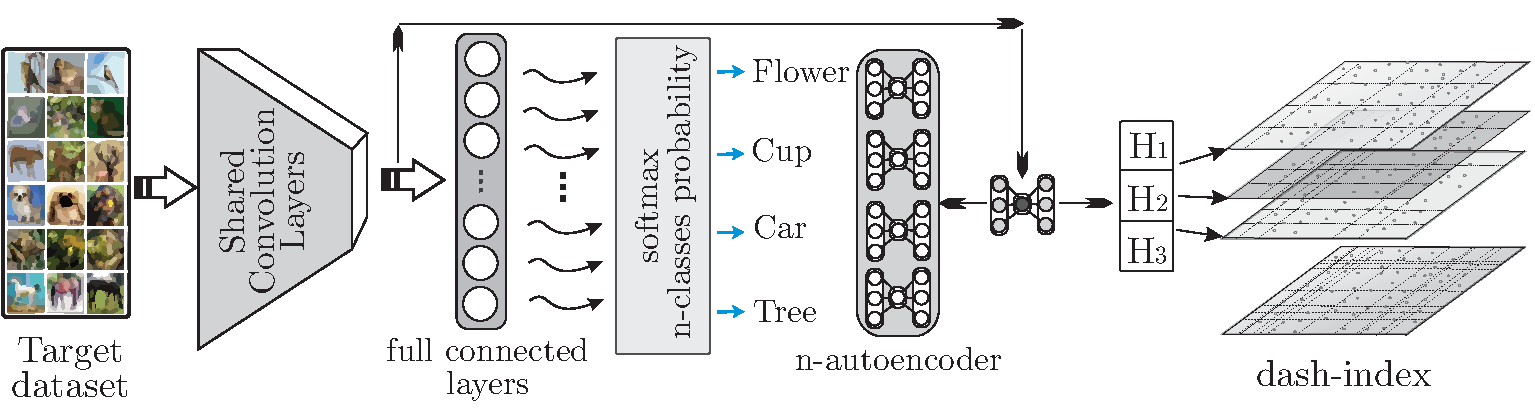
\includegraphics[width=1.7\columnwidth]{dash/DAsh_learning_final.pdf}
\caption{ DAsH: Training and indexing process. } 
\label{fig:dash}
\end{figure*} 		

As it was showed in \cite{citeulike:fractal:encoders} that a successful dimensionality reduction  algorithm projects the data into a feature space with dimensionality close to the fractal dimensionality (FD) of the data in the original space and preserves topological properties.  Thus, to find the target dimensionality ($m$) needed by  autoencoder networks we follow the following  heuristic.  We start with the value at $m_1 = 2^2$, compute the FD of the new space with just that, then increment  value at $m_2 = 2^3$, recompute the FD, and continue doing this until some $ t\ (m_t =  2 ^ t)$ where we can see a flattening in the fractal dimension, meaning that more features do not change the fractal dimensionality of the dataset. 

%The images retrieval procedure is using a coarse-to-fine strategy that separates into two logistic components semantic-level retrieval and hashing-level retrieval.


The second step of our procedure is image retrieval via  DAsH. We process the query image  forwarding it through CNN aiming to obtain the strongest $n$ classes. In contrast to existing similarity learning algorithms that learn similarity from the low-level feature, our similarity is the combination of semantic-level and hashing-level similarity. So, the semantic level similarity is computed firstly. After the semantic relevance checking, we will obtain the new queries ($q_1, q_2, ... q_n$) using the strongest  $n$ autoencoders. The query is transformed into new query objects ($q_1, q_2, ... q_n$) which are hashed to locate the appropriate buckets. Once the buckets are located, the relevant candidate set is formed.  Then, the elements in the candidate set are exhaustively analyzed to recover only the objects that satisfy the query condition. This process is performed for each of the $L$ hash tables. This process is illustrated in Figure \ref{fig:qdash}.  
\begin{figure*}[htp]\centering
\label{fig:qdash}
 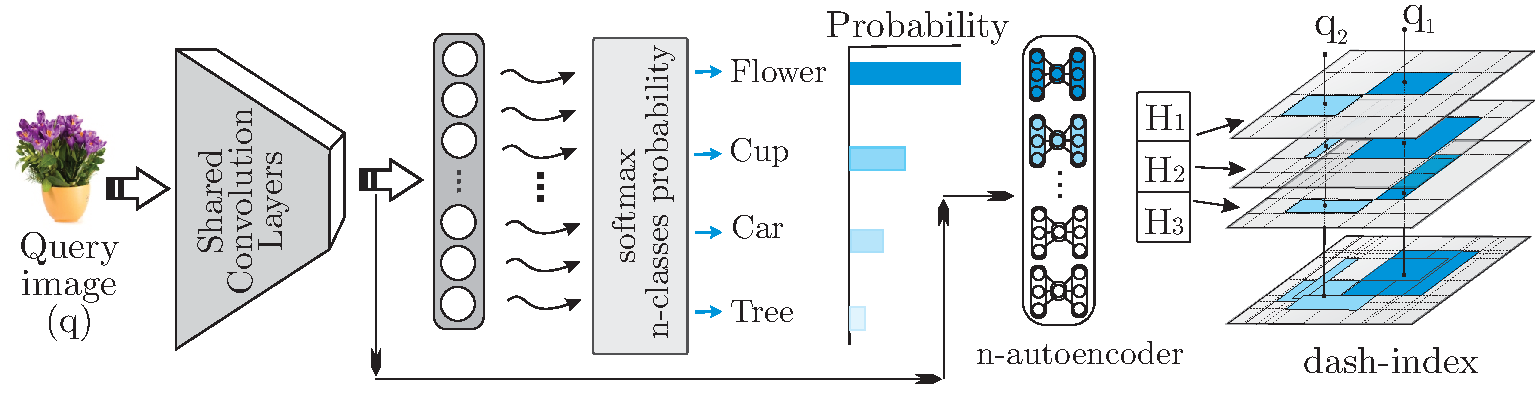
\includegraphics[width=1.70\columnwidth]{dash/DAsh_retrieval_final.pdf} 
\caption{ DAsH. Retrieval process. } 
\end{figure*}


%Our technique changes a one-level hash table into a Multi-level data structure. In each level t the data is organized using distinct numbers of hash functions. The first level of the structure uses $m_1 = 4$ hash functions. The next levels use $m_x =  2 ^ x$, hash functions. The initial value $m_1 = 4$ is the minimum number of hash functions needed to distribute data uniformly into buckets for a standard dataset. Each bucket I can store C objects and a reference list, which keeps references to buckets located in the next level and with a vicinity relation with bucket I. Consecutive levels are thus connected.

%Auto-encoders are known as a class of unsupervised learning algorithms. Unlike supervised algorithms, they do not need label or class information. Autoencoders have been used as a method to pre-train a network and initialize its weights [autoencoderOthman], or as methods of data compression [Le15atutorial].


%A good dimensionality of the data and the closer the intrinsic dimensionality of the data and the closer the intrinsic dimensionality of the dataset in the reduced space is to the intrinsic dimensionality of the dataset in the original space, the between is the classification achieved with the reduced feature set. 



\subsection{Using Fractals to estimate LSH parameters}
	 	 
%The idea to use Correlation Fractal Dimension to compute the LSH parameters take advantage of fractal theory that ensures that a  distance distribution between the elements of the original dataset and a optimal sub-space projection is maintained.  
%In this work we propose a new approach to index CNN features using \ac{LSH} without the data-parameters dependency  problem, exploring the correlations among CNN features by computing the fractal dimension to find the optimal parameter values for LSH.  Then, this values is used to tune LSH scheme during the indexing process  aiming to achieve better accuracy in results with less computational cost during indexing process. 
 
To tune the LSH parameters we used  a property of the   correlation fractal dimension $\mathfrak{D}$, which can  describes statistically a dataset.  Moreover, the correlation fractal dimension $\mathfrak{D}$ can be estimated in linear time as it is depicted in \cite{traina2010fast}. 

We are interested to find out  the resolution scale $log(r)$ at which there are approximately $k$ objects.  Considering the line with slope $\mathfrak{D}$ passing at  a point defined as $  <log (r), log (Pairs(k))>$  the   constant $K_d$ using the Equation \ref{eq:fractal} is:
\begin{eqnarray}\label{eq:fractalk}
	   log(PC(r)) = \mathfrak{D} \times log (r) + K_p \nonumber\\
	   K_p   = log (Pairs (k)) - \mathfrak{D} \times log (r)
\end{eqnarray} 
Considering  another point   $  <log (R), log (Pairs(N))>$, the   constant $K_d$  is defined as :
\begin{equation}\label{eq:fractalN}
    K_d    = log (Pairs(N)) - \mathfrak{D} \cdot log (R) 
\end{equation} 
Now, combining Equations \ref{eq:fractalk}, \ref{eq:fractalN}, we can define  the radius  $r$ as:    	
\begin{equation}\label{eq:fractalR}
  r  =  R \cdot  exp (  \frac{log (Pairs (k)) - log (Pairs(N))}{ \mathfrak{D} } )    
\end{equation}

 Using the last equation \ref{eq:fractalR} we find out that the optimal number of hash functions $m$  for a \acf{LSH} based index configured to retrieve the $k$ nearest neighbors is proportional to the number of pairs at a distance $r$. This has sense, because an average number of $k$ neighbors  are within a given distance $r$.  Then, we define:
\begin{equation}\label{eq:optimalM1}
   m \approx log (PC(r)) 
\end{equation}
 combining  equations \ref{eq:optimalM1} and \ref{eq:fractal} we will obtain that $m \approx \mathfrak{D} \cdot log (r)  $. Experimentally, we confirm out that the optimal  $m$ is:

 \begin{equation}\label{eq:fractalm}
    m = (\left\lceil \mathfrak{D} + 1 \right\rceil  ) \cdot  log (r)
 \end{equation}

 
% The window size have been computed considering experimental results for the most approximate value. As some studies have shown  the window size depends of the query and data distribution \cite{lshtutorial}.  For a dataset $S$ and  query radius  $r$, the window size $w$ for the LSH functions defined above is  $w \approx r$.








\section{SUPERVISED HASHING: A SIMPLE BASELINE}

%This section describes the protocols used in the literature for SSH and SH, and discuss how a simple strategy efficiently solves the corresponding problems.

In this section, we describe the protocols used in the literature for SSH and SH and explain how a simple strategy efficiently solves the similar problems.

\subsection{Evaluation protocols of SSH and SH}

%The task of SSH consists in indexing a dataset of $N$ images $\mathcal{I}_{train}$, of which a subset $\mathcal{I}_{label} \subseteq \mathcal{I}_{train}$ is labeled.  SH is the extreme case $\mathcal{I}_{label} = \mathcal{I}_{train}$. Given an unlabeled query image $q$, the system must return an ordered list of images from the $\mathcal{I}_{train}$. For evaluation purposes, a dataset of queries is given; the labels of the queries as well as all labels in $\mathcal{I}_{train}$ are known to the evaluator, even in the SSH setting, and an image is deemed correct if it has the same label as the query. The performance is measured in terms of precision or mean average precision (mAP), which we now describe. 
SSH consists in index a dataset of $N$ images $\mathcal{I}_{train}$, of which a subset $\mathcal{I}_{label} \subseteq \mathcal{I}_{train}$ is labeled.  But, SH is the extreme case $\mathcal{I}_{label} = \mathcal{I}_{train}$. If we have an unlabeled query image $q$, the system have to return an ordered list of images from the $\mathcal{I}_{train}$. To evaluate, we have a dataset of queries; the evaluator knows all labels of the queries as well as the labels in $\mathcal{I}_{train}$, also in the SSH setting, then an image is considered correct if it and query have the same label. The performance is measured by precision or mean average precision (mAP). 

%Given a query $q$, we first define $\delta (q, i)=1$ if the $i^{th}$ image is correct for $q$, and $0$ otherwise. The precision at (rank) $k$ is given by $P(q,k) = \tfrac{1}{k} {\sum}_{i=1}^{k} \delta (q, i)$. Denoting by $cl(q) = {\sum}_{i=1}^{N} \delta (q, i)$ the total number of correct images in $\mathcal{I}_{train}$, the average precision at $k$ is $AP(q, k) = \tfrac{1}{cl(q)}{\sum}_{i=1}^{k}\delta (q, i) P(q,i)$. The mAP at $k$ (or simply mAP when $k = N$) is the mean AP over all test queries.
Then, given a query $q$, if the $i^{th}$ image is correct for $q$ we define $\delta (q, i)=1$ , and $0$ otherwise. The precision at (rank) $k$ is given by $P(q,k) = \tfrac{1}{k} {\sum}_{i=1}^{k} \delta (q, i)$. Denoting by $cl(q) = {\sum}_{i=1}^{N} \delta (q, i)$ the total number of correct images in $\mathcal{I}_{train}$, and the average precision at $k$ is $AP(q, k) = \tfrac{1}{cl(q)}{\sum}_{i=1}^{k}\delta (q, i) P(q,i)$. The mAP at $k$ (or simply mAP when $k = N$) is the mean AP over all test queries.

\subsection{Retrieval through class probability estimation}

%The information retrieval \cite{doi:10.1108/eb026647} and learning to rank that the optimal prediction for precision at $k$ is given by ranking items $x \in \mathcal{I}_{train}$ n according to their probability of being correct for the query. This result extends to the optimization of $mAP$.

The information recovery \cite{doi:10.1108/eb026647} and learning to rank that the best prediction for precision at $k$ is given by placing items $x \in \mathcal{I}_{train}$ n according to their probability of being correct for the query. This result extends to the optimization of $mAP$.
\\
%\textbf{Optimal ranking for SH.} In the specific setup of SH where the system knows the labels of the images in $\mathcal{I}_{train}$, the probability that an image $x$ with label $y$ is correct is the probability $\mathbb{P}(y\mid q)$ that the query image has label $y$. The important point here is that the probability of $x$ being correct for $q$ only depends on the label of $x$. Thus, ordering the $C$ labels so that $\mathbb{P}(y\mid q)\geq \dots \geq\mathbb{P}(c_C\mid q)$,the optimal ranking is to return all images of $\mathcal{I}_{train}n$ with label $c_1$ first, followed by all images with label $c_2$, and so on.
\textbf{Optimal ranking for SH.} In the particular setup of SH where the system knows the labels of the images in $\mathcal{I}_{train}$, the probability that a picture $x$ with label $y$ is correct is the likelihood $\mathbb{P}(y\mid q)$ that the query image has label $y$. The important point in this part is that the probability of $x$ being correct for $q$ only depends on the label of $x$. Thus, ordering the $C$ labels so that $\mathbb{P}(y\mid q)\geq \dots \geq\mathbb{P}(c_C\mid q)$, the best ranking is to return the complete dataset of $\mathcal{I}_{train}n$ with label $c_1$ first, followed by all the pictures with label $c_2$, and so on.
\\
\begin{comment}
In practice, $\mathbb{P}(.\mid q)$ is unknown, but we can train a classifier
on $\mathcal{I}_{label} = \mathcal{I}_{train}$ which outputs probability estimates $\hat{\mathbb{P}}(c\mid q)$ for every label $c$, and compute the optimal ranking according to $\hat{\mathbb{P}}(c\mid q)$ Such probability estimates are given by,
e.g., multiclass logistic regression or a Convolutional Neural
Network (CNN) with a softmax output layer. Labels of $ \mathcal{I}_{train}$
are stored on [$log2 (C)$] e bits or in an inverted file.
\end{comment}

In practice, $\mathbb{P}(.\mid q)$ is unfamiliar, but we can train a classifier on $\mathcal{I}_{label} = \mathcal{I}_{train}$ which outputs probability con predict $\hat{\mathbb{P}}(c\mid q)$ for every label $c$, and process the optimal ranking according to $\hat{\mathbb{P}}(c\mid q)$ Such probability estimates are shown by, e.g., multiclass logistic regression or a Convolutional Neural
Network (CNN) with a softmax output layer. Labels of $ \mathcal{I}_{train}$
are stored on [$log2 (C)$] e bits or in an inverted file

\\\\
%\textbf{Relationship between classification accuracy and ranking performance.} If we denote the classification accuracy as $p$, then the resulting mAP is at least $p$. When the classifier predicts the class of $q$ correctly, all images of that class will be ranked first and the resulting AP($q$) is $1$; this happens on a proportion $p$ of the queries. So, the classification accuracy is a lower bound on the mAP.

\textbf{Relationship between classification accuracy and ranking performance.} If we show the classification accuracy as $p$, then the resulting $mAP$ is at least $p$. When the classifier foretells the class of $q$ properly, all images of that class will be ranked first, and the resulting AP($q$) is $1$; this happens on a proportion $p$ of the queries. So, the classification accuracy is a lower bound on the mAP.
\\\\
%\textbf{Optimal ranking for SSH.} In the more general setup of SSH, we do not know the label of some images in $\mathcal{I}_{train}$. Yet, considering the (true) conditional label probabilities $\mathbb{P}(c\mid q)$ and $\mathbb{P}(c\mid x)$, the probability that $x$ is correct for $q$ is given by $\sum_{c=1}^C \mathbb{P}(c\mid q) \mathbb{P}(c\mid x) $ it is the probability that both q and x have the same label, assuming conditional independence of the labels of the query and the image. Notice that this is the dot product between the conditional label probability vectors of $q$ and $x$.Then, given probability estimates $\hat{\mathbb{P}}$  for the labels of queries and images, which are obtained on $\mathcal{I}_{label}$, we consider two retrieval algorithms:
\textbf{Optimal ranking for SSH.} In the more general setup of SSH, we do not know the label of some images in $\mathcal{I}_{train}$. Yet, considering the (real) probabilities $\mathbb{P}(c\mid q)$ and $\mathbb{P}(c\mid x)$, the probability that $x$ is correct for $q$ is given by $\sum_{c=1}^C \mathbb{P}(c\mid q) \mathbb{P}(c\mid x) $ it is the probability that both q and $x$ have the same label, assuming conditional self-sufficiency of the labels of the query and the image. Notice that this is the dot product between the dependent label probability vectors of $q$ and x$. Then, given probability measures $\hat{\mathbb{P}}$  for the labels of queries and images, which are taken on $\mathcal{I}_{label}$, we consider two retrieval algorithms:

\\\\
\begin{itemize}
%\item \textbf{Classifier topline: }: For each image $x$of $\mathcal{I}_{train}$, store a vector $u(x)$ equal to either (1) the one-hot encoding vector of the label of $x$ if $x \in \mathcal{I}_{label}$, or (2) the full conditional probability vector  $\hat{\mathbb{P}}(.\mid x)$). Rank images $x$ according to the dot product $\langle\hat{\mathbb{P}}(.\mid q), u(x)\rangle$  This strategy corresponds to the optimal strategy, but requires storing the probability vectors for images in $\mathcal{I}_{train} \backslash \mathcal{I}_{label}$

\item \textbf{Classifier topline: }: For each image $x$of $\mathcal{I}_{train}$, saves a vector $u(x)$ equal to either (1) the one-hot encoding vector of the label of $x$ if $x \in \mathcal{I}_{label}$, or (2) the full  vector  $\hat{\mathbb{P}}(.\mid x)$). Rank images $x$ according to the dot product $\langle\hat{\mathbb{P}}(.\mid q), u(x)\rangle$  This strategy corresponds to the best strategy, but needs to save the probability vectors for each image in $\mathcal{I}_{train} \backslash \mathcal{I}_{label}$

%\item \textbf{Classifier hashed: } Here we hash the conditional probability vector. The first hashing method that we evaluate, is the one-hot strategy, which stores the index of the maximal activation on $\left \lceil log_2(C) \right \rceil$ bits. This approach, denoted \textbf{Classifier+one-hot} in what follows, returns all images of the strongest class first. The second encoding, referred to as Classifier+LSH, is locality-sensitive hashing (LSH) with tight frames \cite{jegou2012anti}, a simple non data adaptive hashing scheme. This LSH method produces binary vectors that are compared with Hamming distances. Therefore it can be used as drop-in replacements for the competing binary encoding methods.

\item \textbf{Classifier hashed: } Here we hash the probability vector. The first hashing method that we evaluate, is the one-hot strategy, which saves the index of the maximal activation on $\left \lceil log_2(C) \right \rceil$ bits. This approach, expressed \textbf{Classifier+one-hot} in what results, returns all images of the strongest class first. The second encoding, referred to as Classifier+LSH, is locality-sensitive hashing (LSH) with tight frames \cite{jegou2012anti}, a simple non data adaptive hashing scheme. This LSH method provides binary vectors that are compared with Hamming distances. Consequently it can be used as drop-in replacements for the competing binary encoding methods.
\end{itemize}

















\section{How should we evaluate supervised hashing?}

\subsection{HASHING FOR NEAREST NEIGHBOR SEARCH}
Compress a set of vectors $(x_i)^{b}_{i=1}, x_i \in \mathbb{R}^{d}$
\begin{figure}[htp]
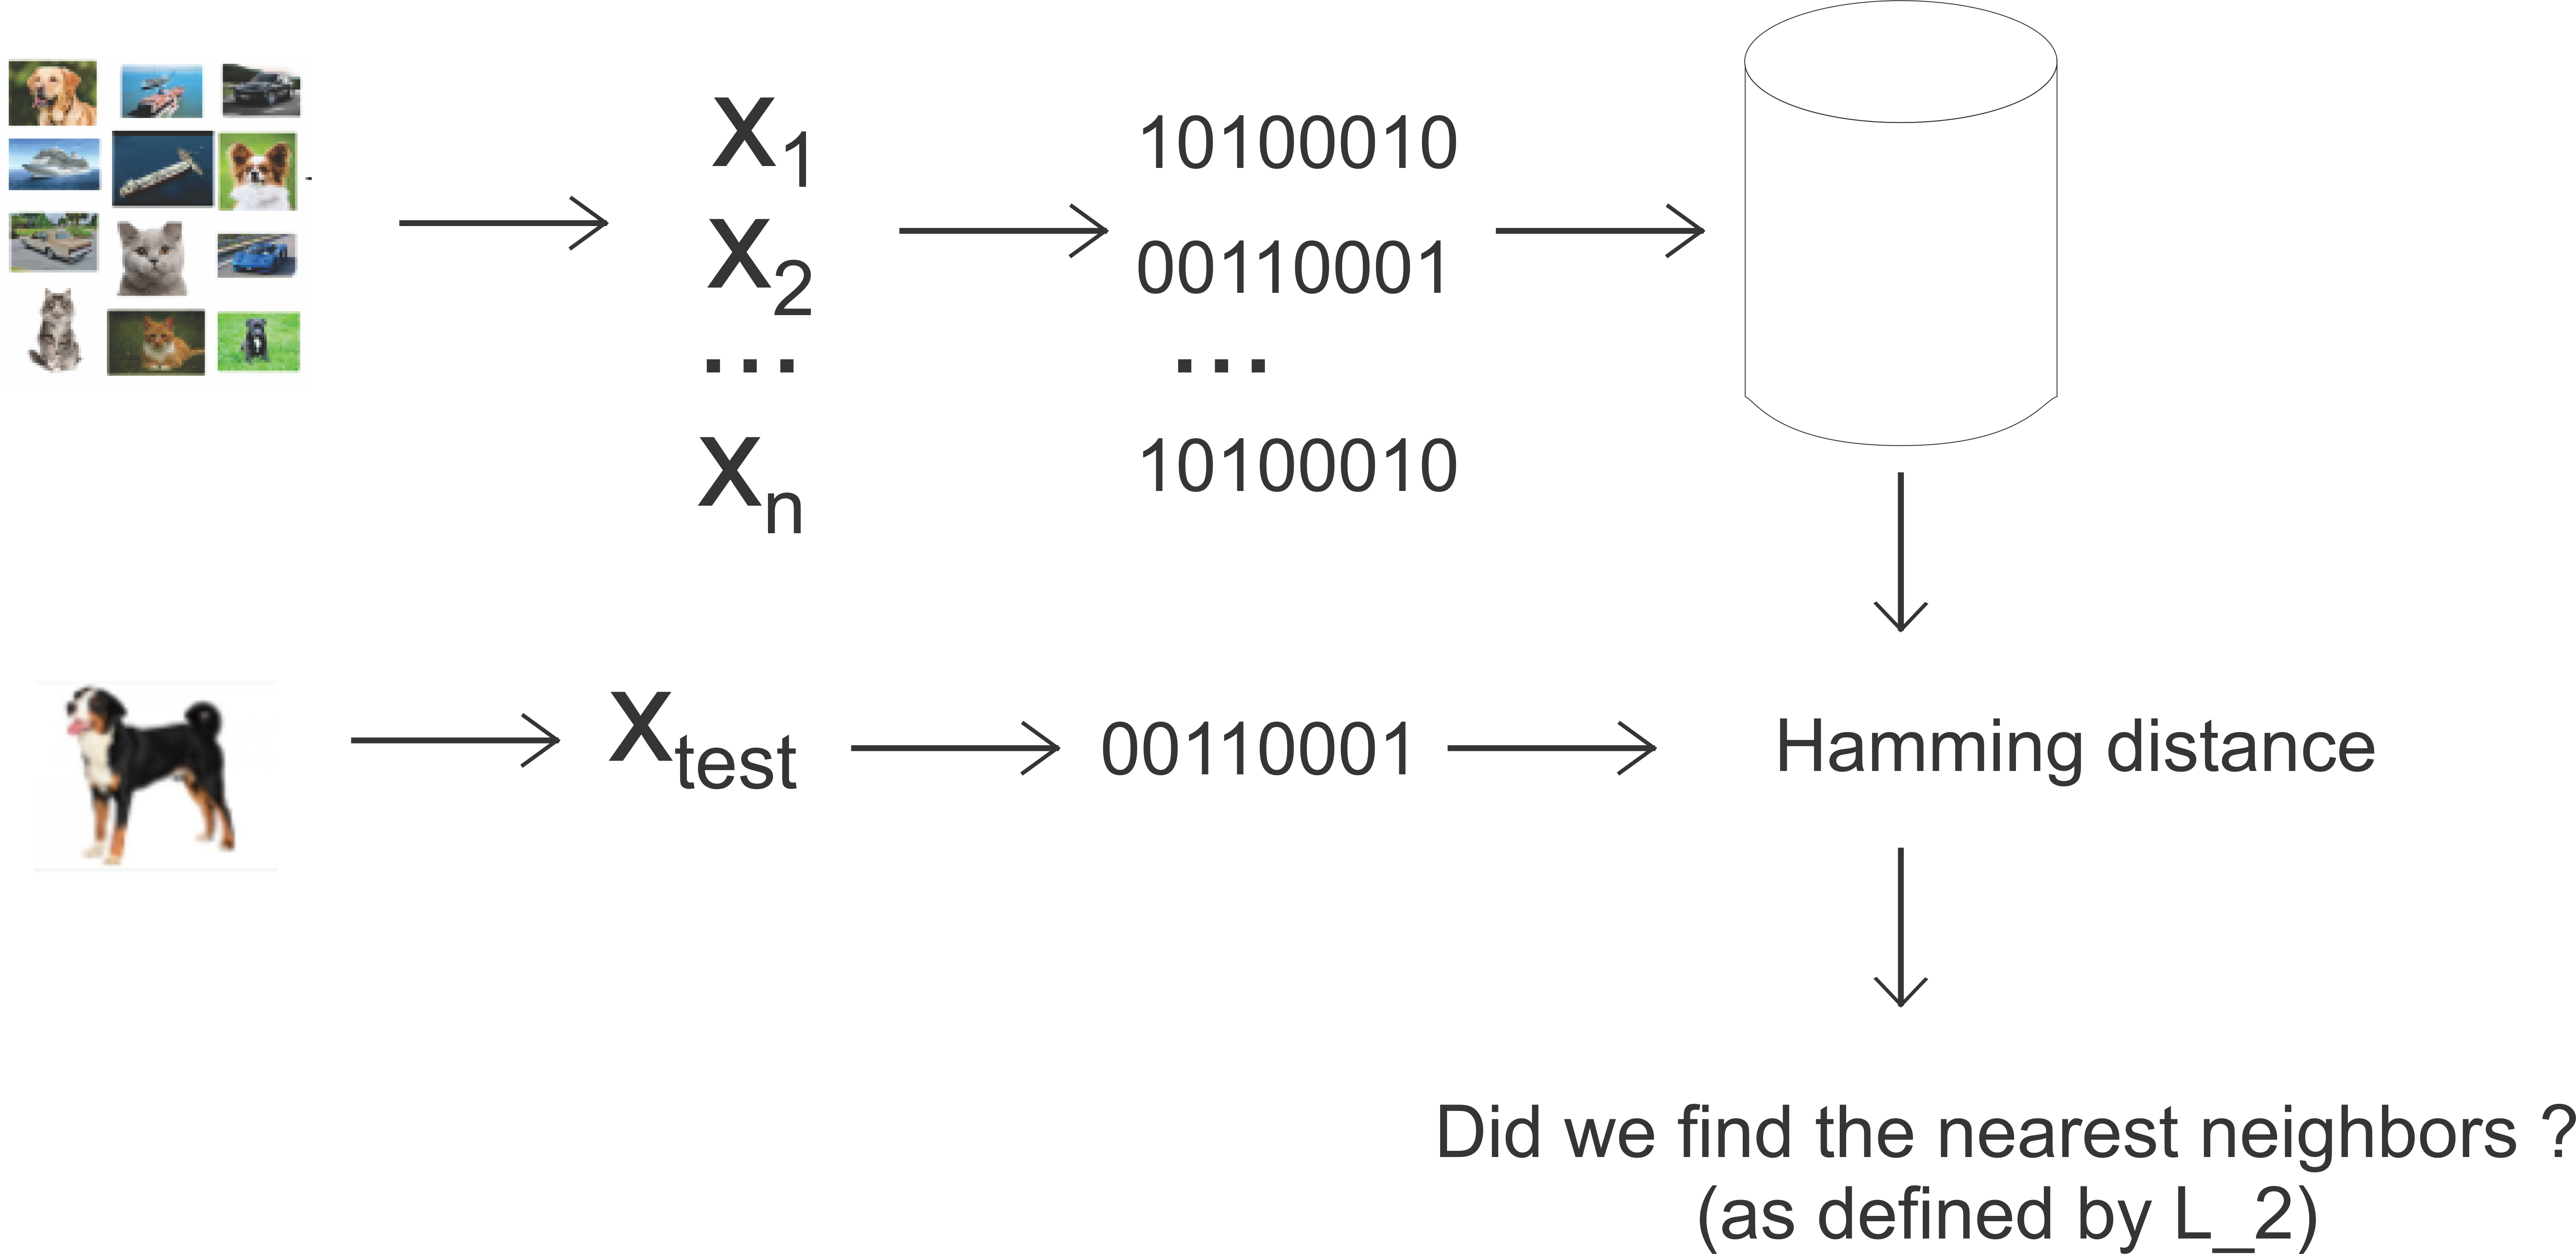
\includegraphics[width=8cm]{dash/11.PNG}
\centering
\end{figure}
 
\subsection{SUPERVISED HASHING}
Compress a set of vectors and their labels  $((x_i,y_2))^{n}_{i=1}, x_1\in \mathbb{R}^{d}, y_1 \in \{1,...,L\} $
\begin{figure}[htp]
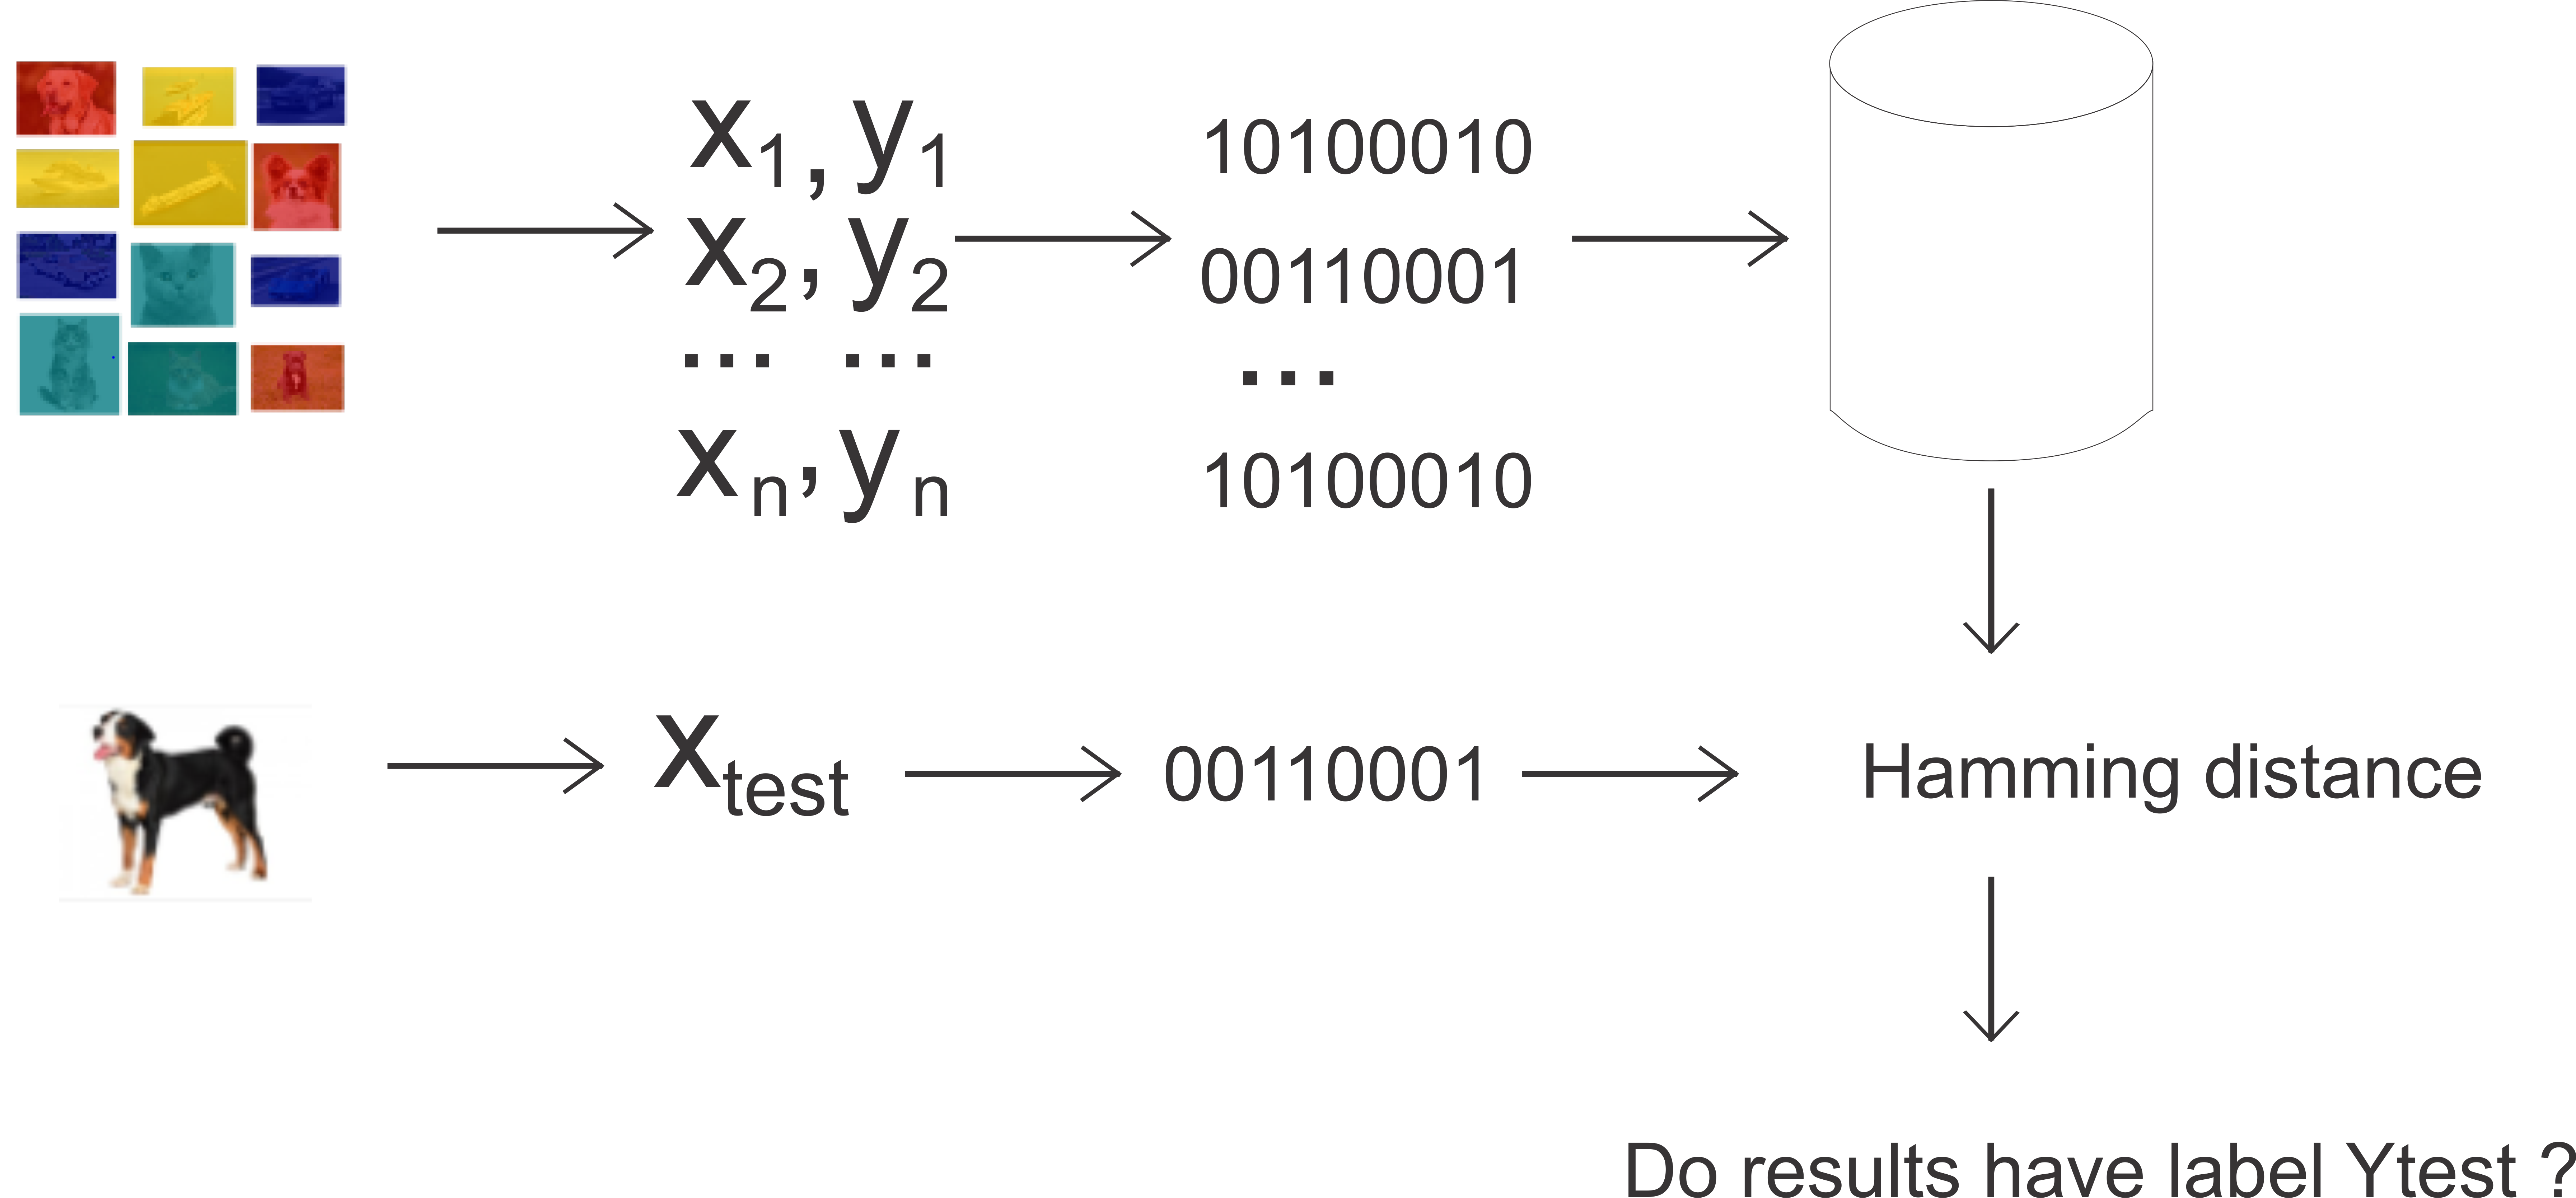
\includegraphics[width=8cm]{dash/12.png} 
\centering
\caption{ HASHING FOR NEAREST NEIGHBOR SEARCH } 
\end{figure}

\begin{itemize}
\item Supervised hashing $[1, 2]$: labels $y$ known for all $x$ in the reference set
\item Semi-supervised hashing $[3, 4]$: labels $y$ known for only $n_label$ samples
\end{itemize}

\subsection{WHY NOT JUST ENCODE THE CLASS ID?}
Supervised hashing with classification baseline
\begin{itemize}
\item Trivial binary encoding of the class id,$ e.g. y=9 \rightarrow 1001$
\centering

\begin{eqnarray}
\cancel{x_1}, y_1  & & 1001    \\
\cancel{x_2}, y_2  & \rightarrow & 1001   \\
\dots  & & \dots \\
\cancel{x_n}, y_n  & & 0011
\end{eqnarray}
\item Train classifier on pairs $(x_1, y_1),  \dots ,(x_n; y_n)$ and predict $y_test$ with the classifier
\item Guaranteed performance: $mAP \geq$ classifier accuracy
\end{itemize}

\subsection{EXTENSION TO SEMI-SUPERVISED HASHING}
\begin{equation}
\begin{split}
	\mathbb{P}(x\;correct for\; q) & = \sum_{j=label} \mathbb{P}(j\mid x)\mathbb{P}(j\mid q)  \\
	&=(\mathbb{P}(j\mid x),\mathbb{P}(j\mid q))  \\
	&=\underbrace{(\hat{\mathbb{P}}(j\mid x)}_{classifier},\hat{\mathbb{P}}(j\mid q))  \\
\end{split}
\end{equation}
\begin{itemize}
    \item Train $\hat{\mathbb{P}}$ on labelled images
    \item Compute $\hat{\mathbb{P}}(\cdot\mid x) \in\left[0,1\right]^{L}$ for $x$ unlabelled
    \item Compress $\hat{\mathbb{P}}(\cdot\mid x)$ with one-hot / LSH
\end{itemize}

\begin{table}[]
\centering
\caption{Results on CIFAR-10}
\label{my-label}
\begin{tabular}{|l|l|l|l|l|l|}
\hline
Features & $n_label$ & $n_anchors$ & Method                                                                                    & bits                                                         & mAP                                                                           \\ \hline
GIST     & 59,000    & 1,000       & \begin{tabular}[c]{@{}l@{}}SQ{[}1{]}\\ SQ{[}1{]}\\ One-hot\end{tabular}                   & \begin{tabular}[c]{@{}l@{}}64\\ 128\\ 4\end{tabular}         & \begin{tabular}[c]{@{}l@{}}0.704\\ 0.712\\ 0.762\end{tabular}                 \\ \hline
GIST     & 5,000     & 1,000       & \begin{tabular}[c]{@{}l@{}}SDH{[}3{]}\\ One-hot\\ LSH\\ Topline\end{tabular}              & \begin{tabular}[c]{@{}l@{}}64\\ 4\\ 64\\ -\end{tabular}      & \begin{tabular}[c]{@{}l@{}}0.402\\ 0.377\\ 0.430\\ 0.578\end{tabular}         \\ \hline
GIST     & 1,000     & 300         & \begin{tabular}[c]{@{}l@{}}KSH{[}4{]}\\ KSH{[}4{]}\\ One-hot\\ LSH\\ Topline\end{tabular} & \begin{tabular}[c]{@{}l@{}}12\\ 48\\ 4\\ 48\\ -\end{tabular} & \begin{tabular}[c]{@{}l@{}}0.232\\ 0.284\\ 0.270\\ 0.309\\ 0.350\end{tabular} \\ \hline
DEEP     & 50,000    & -           & \vdots                                                                                    & \vdots                                                       & \vdots                                                                        \\ \hline
AlexNet  &           &             & \begin{tabular}[c]{@{}l@{}}DSH{[}2{]}\\ DSH{[}2{]}\\ One-hot\end{tabular}                 & \begin{tabular}[c]{@{}l@{}}12\\ 48\\ 4\end{tabular}          & \begin{tabular}[c]{@{}l@{}}0.616\\ 0.621\\ 0.870\end{tabular}                 \\ \hline
\end{tabular}
\end{table}
\begin{table}[]
\centering
\caption{Results on ImageNet}
\label{my-label}
\begin{tabular}{llll}
Features & Method    & bits & mAP@1500 \\
VGG      & SQ{[}1{]} & 128  & 0.620    \\
VGG      & one-hot   & 10   & 0.664   
\end{tabular}
\end{table}

\textbf{Encoding schemes}
\begin{itemize}
\item One-hot:$(0.15,0.07,0.08,\textbf{0.7})\rigtharrow 3 \rigtharrow 0011$ 
\item LSH:$(0.15,0.07,0.08,0.7)\rigtharrow (sign(w_i^T \cdot v + b_i))_{i=1}^{n_bits}$ 
\item Top line: no compression
\end{itemize}

\subsection{HOW CAN WE AVOID THIS BIASED PROTOCOL?}
\ref{fig:13}.  
\begin{figure*}[htp]\centering
\label{fig:13}
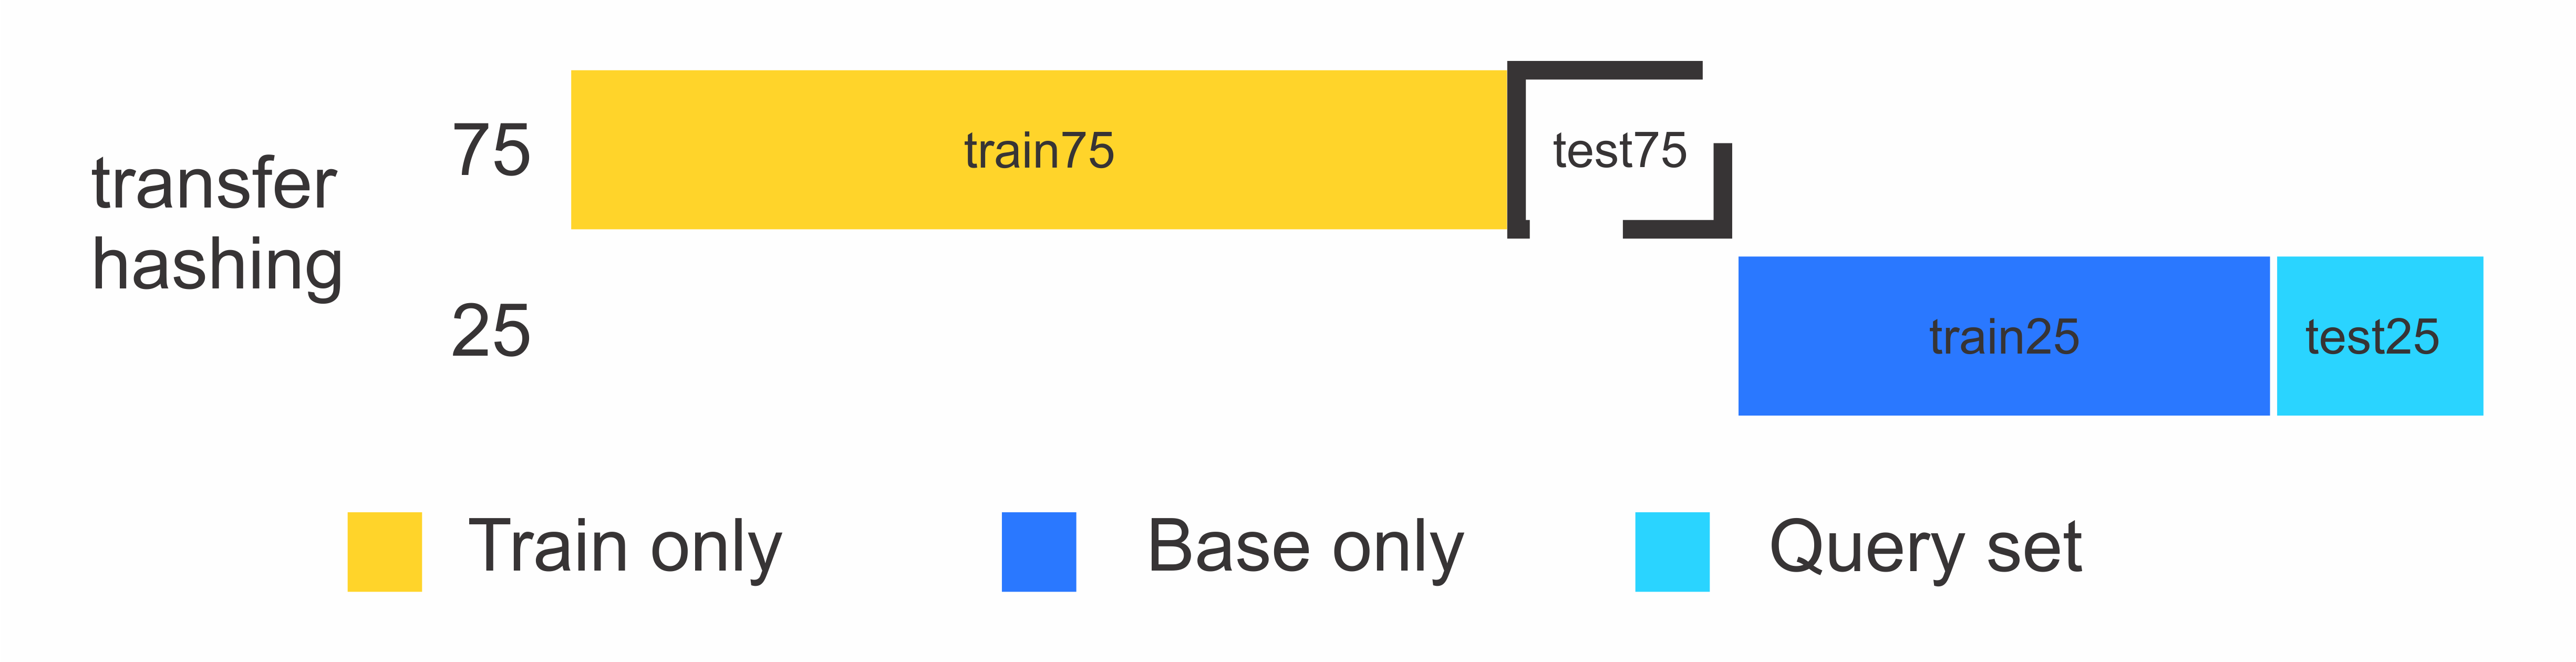
\includegraphics[width=8cm]{dash/13.png} 
\end{figure*}

\begin{itemize}
\item Test on classes \textbf{never seen at train time}
\itemSplit classes in 4 folds, each with 25\% of classes,Both setups:
    \begin{itemize}
    \item Train hash functions on train75
    \item Encode train25 with hash functions
    \end{itemize}
\item \textbf{Setup 1: Retrieval with hash codes}
    \begin{itemize}
    \item Use train25 as reference set
    \item Use test25 as queries
    \end{itemize}
\item \textbf{Setup 2: Classification on hash codes}
    \begin{itemize}
    \item Train classifier using train25 labels
    \item Evaluate accuracy on test25
    \end{itemize}
\end{itemize}

\subsection{UNSUPERVISED BASELINE FOR PROPOSED PROTOCOL}
\begin{itemize}
\item \textbf{Experimental setting}
    \begin{itemize}
    \item Experiments with CIFAR-10 using AlexNet
    \item Unsupervised PQ codes [5] with 4 bytes
    \end{itemize}
\item \textbf{Setup 1: Retrieval with hash codes}
    \begin{itemize}
    \item PQ codes with asymmetric comparison
    \item Higher layers are better
    \item 4 bytes enough for most of performance
    \item Inner product on softmax gets the best result
    \end{itemize}
\item \textbf{Setup 2: Classification on hash codes}
    \begin{itemize}
    \item Drop in accuracy due to encoding
    \item Lower layers more generic$\rightarrow$better accuracy
    \item Lower layers high dimensional$\rightarrow$larger gap between PQ and full vector
    \item $\rightarrow$ Trade-off encoding/accuracy
    \end{itemize}
\end{itemize}

















\section{EVALUATION PROTOCOLS}

In this section, we describe the two evaluation tasks proposed in \cite{sablayrolles2016should}, namely retrieval of unseen classes, and transfer learning to new classes. They correspond to application cases on large datasets. The two protocols differ only in the evaluation metric: ranking versus class accuracy.

\textbf{Dataset definition.} at test time we use separate classes from a standard classification dataset. When learning the hashing function $75\%$ of the classes are assumed to be known, and the $25\%$ remaining classes are used to evaluate the encoding/hashing scheme. We call train75/test75 the train/test images of the $75\%$ classes and train25/test25 the remaining ones.

\textbf{Protocol 1: Retrieval of unseen classes}, to index train25 and use test25 as queries, we use the hashing scheme. We use the labels of train25 for evaluation only. This setup is like an instance search approach except that the class labels give the ground-truth. The train75 - train25 - test25 split is the supervised equivalent of the learn - database - query split in unsupervised hashing. 

\textbf{Protocol 2: Transfer learning, } the authors proposed to train a new CNN from scratch with the same structure as the top of the original network, using the stored train25 descriptors. The goal is to maximize the transfer accuracy on test25. 

\section{Experiments}

In this section, we are interested in answering the following question: (a) How accurate is our model in estimating the LSH parameters using the fractal dimension; (b) How does our DAsH method  improve the other LSH implementations in terms of \textit{querying performance} and \textit{precision}. The performance of DAsH method was compared to  two   well-known approximate search methods, namely  Multi-probe LSH \cite{multiprobe}, LSH-Forest \cite{lshforest}, ITQ \cite{itq}, and LOPQ \cite{lopq}. All of the experiments were performed on a workstation with Intel core i7  3.0Ghz (12 cores) CPU and 64Gb RAM which is supplied with four Geforce GTX 1080 GPU with 8Gb VRAM each one.
 
We first conduct experiments on eight  widely used datasets using hand-crafted features (AUDIO, CITIES, EIGENFACES, HISTOGRAMS, MGCOUNTY, RANDOMWALK, SYNTH16D, SYNTH6D, VIDEO)\footnote{\url{https://github.com/joselhuillca/fractal_dataset}} to evaluate our proposed  method for   estimating the LSH parameters. Beside hand-crafted features, we also show the effectiveness of our methods when deep features   are extracted by the deep Convolutional Neural Networks (CNN),  we conduct this experiment on three datasets (MNIST\footnote{\url{http://yann.lecun.com/exdb/mnist/}}, CIFAR-10\footnote{\url{https://www.cs.toronto.edu/~kriz/cifar.html}}, SVHN\footnote{\url{http://ufldl.stanford.edu/housenumbers/}}) to evaluate our in terms of querying performance,  meap average precision (mAP), and precision. The following describes the details of the experiments and results. 













\subsection{Experiment 1: Tunning LSH Parameters}

LSH based methods report efficient results when adequate values for $m$ (number of hash functions) are chosen. To evaluate the effectiveness of the presented approach to tune the LSH parameters using fractal dimension, we worked on a variety of synthetic and real dataset. Table \ref{table:lshparams} summarizes the main features and parameters of the datasets, including the number of elements $N$, number of attributes $d$,   their intrinsic (fractal) dimension $\mathfrak{D}$, the LSH parameters computed using two approaches: the Andoni \footnote{\url{http://www.mit.edu/~andoni/LSH/}} algorithm and our proposal based on fractal dimension, and the total computation time for tune the LSH index (in seconds).  The experiment results for the number of hash functions $m$  show that the estimations given by Equation \ref{eq:fractalm} are comparable with those obtained with the E2LSH algorithm proposed by Andoni using up to $10X$ less time.
 
\begin{table*}[ht]
\caption{Optimal LSH Params using exhaustive e2lsh and the fractal based method.}
\label{table:lshparams}
\centering
\begin{footnotesize}
\begin{tabular}{c|r|r|r|r|r|r|r|r|r|r|}
    \cline{2-11}
    & \multicolumn{ 2}{|c|}{{\bf dataset}} & \multicolumn{ 3}{|c|}{{\bf fractal params}} & \multicolumn{ 2}{|c|}{{\bf e2lsh}} & \multicolumn{ 3}{|c|}{{\bf fractalsh}}  \\
    \cline{2-11}
    & \multicolumn{1}{c|}{$N$}    & \multicolumn{1}{c|}{$d$} & \multicolumn{1}{c|}{$\mathfrak{D}$}    & $log(R)$ & $log(CR)$   & $m$ & \multicolumn{1}{c|}{$time(s)$}    & \multicolumn{1}{c|}{$r$}  & $m$ & \multicolumn{1}{c|}{$time(s)$} \\
    \hline
\multicolumn{1}{|c|}{\bf audio}                 & 54387                 & 192      & 6.49     & -1.30      & 17.00       & \cellcolor[HTML]{f2f2f2}18                        & \cellcolor[HTML]{f2f2f2}64.20     & 0.14  & \cellcolor[HTML]{DFDFDF}16                    & \cellcolor[HTML]{DFDFDF}12.68                   \\
\multicolumn{1}{|c|}{\bf cities}                & 5507                  & 2        & 2.36     & 2.30       & 16.00       & \cellcolor[HTML]{f2f2f2}8                         & \cellcolor[HTML]{f2f2f2}16.45      & 4.16  & \cellcolor[HTML]{DFDFDF}6                     & \cellcolor[HTML]{DFDFDF}0.81                    \\
\multicolumn{1}{|c|}{\bf eigenfaces}            & 11900                 & 16       & 4.25     & -1.40      & 18.00       & \cellcolor[HTML]{f2f2f2}12                        & \cellcolor[HTML]{f2f2f2}42.28      & 0.13  & \cellcolor[HTML]{DFDFDF}13                    & \cellcolor[HTML]{DFDFDF}1.57                    \\
\multicolumn{1}{|c|}{\bf histograms}            & 4247                  & 256      & 2.50     & -0.81      & 16.01       & \cellcolor[HTML]{f2f2f2}6                         & \cellcolor[HTML]{f2f2f2}15.62      & 0.22  & \cellcolor[HTML]{DFDFDF}7                     & \cellcolor[HTML]{DFDFDF}6.12                    \\
\multicolumn{1}{|c|}{\bf mgcounty}              & 27282                 & 2        & 1.81     & 0.70       & 19.00       & \cellcolor[HTML]{f2f2f2}4                         & \cellcolor[HTML]{f2f2f2}87.96      & 0.27  & \cellcolor[HTML]{DFDFDF}4                     & \cellcolor[HTML]{DFDFDF}1.13                     \\
\multicolumn{1}{|c|}{\bf randomwalk}            & 10000                 & 1024     & 5.52     & 2.80       & 15.00       & \cellcolor[HTML]{f2f2f2}16                        & \cellcolor[HTML]{f2f2f2}50.60     & 10.16 & \cellcolor[HTML]{DFDFDF}17                    & \cellcolor[HTML]{DFDFDF}10.60                   \\
\multicolumn{1}{|c|}{\bf synth16d}              & 10000                 & 16       & 8.36     & -1.40      & 17.00       & \cellcolor[HTML]{f2f2f2}20                        & \cellcolor[HTML]{f2f2f2}27.20     & 0.18  & \cellcolor[HTML]{DFDFDF}18                    & \cellcolor[HTML]{DFDFDF}7.51                   \\
\multicolumn{1}{|c|}{\bf synth6d}               & 10000                 & 6        & 4.95     & -1.40      & 17.00       & \cellcolor[HTML]{f2f2f2}12                        & \cellcolor[HTML]{f2f2f2}28.16      & 0.14  & \cellcolor[HTML]{DFDFDF}12                    & \cellcolor[HTML]{DFDFDF}6.47                    \\
\multicolumn{1}{|c|}{\bf video}                 & 79094                 & 50       & 7.73     & -1.40      & 21.00       & \cellcolor[HTML]{f2f2f2}16                        & \cellcolor[HTML]{f2f2f2}1205.73     & 0.13  & \cellcolor[HTML]{DFDFDF}19                    & \cellcolor[HTML]{DFDFDF}92.54                   \\ 
\hline
\end{tabular}
\end{footnotesize}
\end{table*}
%LSH based methods report efficient results when adequate values for $m$ (number of hash functions), $L$ (number of indexes), $T$ (number of probes for Multi-probe LSH) are chosen.   The LSH parameters ($m$ and $L$) used in this experiment were tuned according to the implementation of Exact Euclidean LSH (E2LSH) \footnote{\url{http://www.mit.edu/~andoni/LSH/}}. The tuning parameter $m$ is chosen as a function of the dataset to minimize the running time  of a query  while the space requirement is within the memory bounds. \Correction{$L$ is given by $L = m(m-1)/2$}.  And $T$ is defined using the following reasoning: The original LSH uses $L$ projections to respond a query. The Multi-probe LSH requires fewer indexes to respond a query (say $L'$, $L' < L$). Thus, the number of projections used by the Multi-probe LSH is $L' \times T$ which should be approximately equal to $L$.   The query range for LSH and Multi-probe LSH was set to $k = 1000$\%.

 

%\begin{figure}[ht]
%\includegraphics[width=0.3\columnwidth]{plots/mnist_128.pdf}
%\includegraphics[width=0.3\columnwidth]{plots/svhn_256.pdf}
%\includegraphics[width=0.3\columnwidth]{plots/cifar10_512.pdf} 

%\caption{Precision-recall curves of euclidean ranking for MNIST, SHVN and CIFAR-10 Datasets. }
%\label{fig:knn_1}
%\end{figure} 


\subsection{Retrieval Performance} % OK
 The aim of this experiment is to measure the total time   spent  retrieving the $k$-nearest neighbor objects. The data structures being compared were tested with an specific values for queries. Thus we use   $k=1000$   when compute the Mean Average Precision($mAP$) metric and $k=25$ when compute the  precision metric $(P (\%))$.
\begin{table*}[ht]
\caption{Mean Average Precision(mAP), precision, and cumulative time spent to compute mAP for different methods on the MNIST, SVHN  and CIFAR-10 datasets. }
\label{table:map}
\centering
\begin{footnotesize}
\begin{tabular}{l|c|c|c|c|c|c|c|c|c|}
\cline{2-10}
                                           & \multicolumn{3}{c|}{\textbf{MNIST}}            & \multicolumn{3}{c|}{\textbf{SVHN}}             & \multicolumn{3}{c|}{\textbf{CIFAR-10}}         \\ \cline{2-10} 
                                           & \textbf{mAP} & \textbf{P (\%)} & \textbf{time(s)} & \textbf{mAP} & \textbf{P (\%)} & \textbf{time(s)} & \textbf{mAP} & \textbf{P (\%)} & \textbf{time(s)} \\ \hline
\multicolumn{1}{|l|}{\textbf{MpLSH \cite{multiprobe}}}       & 0.86         & 0.95            & \cellcolor[HTML]{c8c8c8}19.58         & 0.71         & 0.73            & 8.09          & \cellcolor[HTML]{c8c8c8}0.83         & 0.89            & \cellcolor[HTML]{c8c8c8}122.45        \\ \hline
\multicolumn{1}{|l|}{\textbf{ITQ \cite{itq}}}         & 0.87         & 0.95            & 1297.32       & 0.70         & 0.80            & 8411.26       & 0.84         & 0.88            & 1056.83       \\ \hline
\multicolumn{1}{|l|}{\textbf{LOPQ \cite{lopq}}}        & 0.86         & 0.90            & 119.21        & 0.71         & 0.74            & 613.65        & 0.83         & 0.88            & 528.20        \\ \hline
\multicolumn{1}{|l|}{\textbf{LSH-F \cite{lshforest}}}       & 0.85         & 0.96            & 217.33        & 0.61         & 0.78            & 365.90        & 0.86         & 0.89            & 365.47        \\ \hline
\multicolumn{1}{|l|}{\textbf{DAsH (Ours)}} & \cellcolor[HTML]{c8c8c8}0.93         & \cellcolor[HTML]{c8c8c8}0.98            & \cellcolor[HTML]{f2f2f2}20.82         & \cellcolor[HTML]{c8c8c8}0.74         & \cellcolor[HTML]{c8c8c8}0.84            & \cellcolor[HTML]{f2f2f2}10.34         & \cellcolor[HTML]{c8c8c8}0.88         & \cellcolor[HTML]{c8c8c8}0.91            & \cellcolor[HTML]{f2f2f2}125.37        \\ \hline
\end{tabular}
\end{footnotesize}
\end{table*}

Table  \ref{table:map} show the comparison in terms of mean average precision mAP, precision, and total time (in seconds).


\begin{table*}[ht]
\centering
\caption{My caption}
\label{my-label}
\begin{tabular}{|l|r|r|r|r|r|r|r|}
\hline
                     & \multicolumn{6}{c|}{\textbf{SMALL SPACE}}                 & \multicolumn{1}{l|}{\textbf{ORIG. SPACE}} \\ \hline
\multicolumn{8}{|c|}{\textbf{AGNEW}}                                                                                         \\ \hline
\textbf{Dim}         & 16      & 32      & 64      & 128     & 256     & 512     & 8704                                      \\ \hline
\textbf{Fractal Dim} & 4.2656  & 4.5797  & 5.7044  & 20.5952 & 24.7651 & 24.7651 & 30.4943                                   \\ \hline
\multicolumn{8}{|c|}{\textbf{CIFAR10}}                                                                                       \\ \hline
\textbf{Dim}         & 16      & 32      & 64      & 128     & 256     & 512     & 4096                                      \\ \hline
\textbf{Fractal Dim} & 1.4436  & 5.4327  & 7.2287  & 23.2534 & 25.5753 & 25.5753 & 1.6494                                    \\ \hline
\multicolumn{8}{|c|}{\textbf{ISBI}}                                                                                          \\ \hline
\textbf{Dim}         & 16      & 32      & 64      &         &         &         & 4096                                      \\ \hline
\textbf{Fractal Dim} & 11.6047 & 16.1283 & 16.1283 &         &         &         & 16.1283                                   \\ \hline
\multicolumn{8}{|c|}{\textbf{MNIST}}                                                                                         \\ \hline
\textbf{Dim}         & 16      & 32      & 64      & 128     & 256     &         & 800                                       \\ \hline
\textbf{Fractal Dim} & 4.3912  & 4.1542  & 22.5753 & 22.5753 & 22.5753 &         & 22.5753                                   \\ \hline
\multicolumn{8}{|c|}{\textbf{SVHN}}                                                                                          \\ \hline
\textbf{Dim}         & 16      & 32      & 64      & 128     &         &         & 1152                                      \\ \hline
\textbf{Fractal Dim} & 6.5841  & 4.6553  & 28.3359 & 28.3359 &         &         & 28.3359                                   \\ \hline
\end{tabular}
\end{table*}

\section{Conclusions}

In this paper, we presented a new scheme to solve approximate similarity search by supervised hashing called Deep Fractal base Hashing.  Our approach shows the potential of boosting querying operations when a specialized index structure is designed from end-to-end.  Due to the abilities of Fractal theory to find the optimal sub-space of the dataset and the optimal number of hash functions for LSH Index, we are able to find an optimal configuration for learning and indexing process.  Moreover, we defined a novel method, based on fractal theory, which allows us to can find the optimal number of hash functions for  LSH index. We can estimate these parameters in linear time due to it depends on computing fractal dimension. 

We conducted performance studies on many real and synthetic datasets.  The empirical results for LSH parameters show that our method based on fractal theory is comparable with those obtained with the brute-force algorithm using up to $10X$ less time. Moreover, in retrieval performance, the DAsH method was significantly better than other approximate methods, providing up to 8\%  better precision maintaining excellent retrieval times.  %This result demonstrates the potential of boosting querying operations with designing specialized index structures.



% This paper proposes a novel supervised hashing technique,  named  Deep frActal based  Hashing (DAsH),  designed to perform scalable approximate similarity search. The contributions of our work are as follows. First,  we introduce and define a  scheme based on CNN and optimized using fractal theory. To overcome the limitation of large activations on lower layers of CNN (output of the last convolutional layer) we reduce its dimensionality using autoencoders  to the optimal sub-space. Then we index this new representation with LSH scheme.  Second, we present a novel method, based on fractal theory, which allow us to can find the optimal number of hash functions for an approximate similarity search scheme based on LSH.



%considers the linear and multi-level hashing scheme to adjust the number of hash functions and number of buckets needed to index a dynamic set of objects .  Due to the self-adaptive abilities of the multi-resolution index structure we can adapt the data domain parameters during the indexing process.  Additionally, this scheme allows us to exploit the multi-resolution approach to compute the number of probes needed for a specific query. As a consequence, we can speed up the query process as the need of more indexes decreases.




%In this paper, we presented a new scheme to solve approximate similarity search called Adaptive Multi-level Locality Sensitive Hashing. \ConnectDots{Our approach considers the linear and multi-level hashing scheme to adjust the number of hash functions and number of buckets needed to index a dynamic set of objects}.  Due to the self-adaptive abilities of the multi-resolution index structure we can adapt the data domain parameters during the indexing process.  Additionally, this scheme allows us to exploit the multi-resolution approach to compute the number of probes needed for a specific query. As a consequence, we can speed up the query process as the need of more indexes decreases.

%We conducted performance studies on many real and synthetic datasets. The empirical results show that Multi-level LSH outperforms the metric data structures and LSH-based methods by decreasing the query time (number of distance computations) by up to 51\% (72\%) in comparison to the original LSH and 34\% (45\%) in comparison to Multi-probe LSH. Additionally, Multi-level LSH reduces space usage by up to 35\% in comparison to the original LSH and it has similar results in comparison to Multi-probe LSH.  Our results show the self-tuning behavior of our approach during the indexing process offering sub-linear cost for query processing and preserving an acceptable accuracy score. \Correction{Additionally, our experimental studies show that, current state-of-the-art metric trees exhibit exact precision and satisfactory performance and usage space. However, even though LSH methods have a trade-off among space, speed and quality, they are still more effective and faster than metric trees specially in sceneries where the dataset size and dimension are very high. That was expected but not clear in the literature considering that ,in contrast to LSH methods, metric tree structures suffer from the ``curse of dimensionality'' problem. }

%\pgfplotstabletypeset[
%col sep = comma,
%string replace*={_}{\textsubscript},
%every head row/.style={before row=\toprule,after row=\midrule},
%every last row/.style={after row=\bottomrule},
%display columns/0/.style={string type,column name={}}
%]{csv/methods.csv}
    

\bibliographystyle{IEEEtran}
\bibliography{sbc-template}
 

% that's all folks
\end{document}


